\documentclass[12pt]{mwrep}
\usepackage{polski}
\usepackage[utf8]{inputenc}
\usepackage[T1]{fontenc}
\usepackage{times}



\usepackage[margin=20mm, left=30mm]{geometry}

%\usepackage{newtxtext}
%\usepackage{newtxmath}
\usepackage{amsmath}
\usepackage{bm}
\usepackage{mathtools}
\mathtoolsset{showonlyrefs}


\usepackage{tabularx}
\usepackage{array}
\newcolumntype{Y}{>{\centering\arraybackslash}X}
\newcolumntype{Z}{>{\centering\arraybackslash}p}
\usepackage{multirow}
\usepackage[table]{xcolor}
\usepackage{array}
\setlength\arrayrulewidth{1pt}
\newcommand{\x}{\overline{d}}
\usepackage{hyperref}


\renewcommand{\thesection}{{\hspace{-10mm}}\arabic{section}}
\renewcommand{\thesubsection}{{\hspace{-5mm}}\arabic{section}.\arabic{subsection}}

\usepackage{enumitem}
\usepackage{float}
%\usepackage{longtable}
\usepackage{graphicx}
%\usepackage{rotating}
%\usepackage{subcaption}

\newcommand{\code}[1]{\texttt{#1}}

\newcommand{\dd}{\text{d}}

%%%%%%%%%%%%%%%%%%%%%%%%%%%%%% Malec - preambuła
\usepackage{amssymb, amsfonts}






%%%%%%%%%%%%%%%%%%%%%%%%%%%%%% Budnik - preambuła
\newcommand{\indep}{\perp \!\!\! \perp}
%\usepackage{titlesec}
%\titleclass{\subsubsection}{straight}[\subsection]
%\newcounter{\subsubsection}[subsubsection]
%\renewcommand{\thesubsubsection}{{\hspace{-2mm}}\arabic{section}.\arabic{subsection}.\arabic{subsubsection}}
%\usepackage{unicode-math}
%\usepackage{dutchcal}
%\usepackage{fontspec}
%\usepackage{unicode-math}
%\setmathfont{Asana Math}
\usepackage{subfig}








\begin{document}%%%%%%%%%%%%%%%%%%%%%%%%%%%%
	\begin{center}
		{\Large\textbf{Symulacje Komputerowe}}
	\end{center}
	\begin{center}
		Raport: \textbf{1}
	\end{center}
	
	\noindent Temat sprawozdania \dotfill \textbf{Coś kreatywnego} \dotfill\dotfill\\
	Nazwisko i Imię prowadzącego kurs \dotfill \textbf{dr Michał Balcerek} \dotfill\dotfill	\newline\newline
	
	
	\noindent\begin{tabularx}{\textwidth}{|X |X|}
		\hline
		Wykonawca: & \\\hline
		\begin{center}
			Imię i Nazwisko,\\ nr indeksu
		\end{center} &  \begin{center}
			Kacper Budnik, 262286\\
			Szymon Malec, 262276
		\end{center}\\\hline
		Wydział & Wydział matematyki, W13 \\\hline
		Termin zajęć: & Wtorek,\vphantom{ $11^{1^{5}}$} $11^{15}$\\\hline
		Numer grupy ćwiczeniowej & T00-70d \\\hline
		Data oddanie sprawozdania: & \today \\\hline
		\textbf{Ocena końcowa} &\\\hline
		
	\end{tabularx}\newline\newline
	
	
	\noindent\textbf{Adnotacje dotyczące wymaganych poprawek oraz daty otrzymania poprawionego sprawozdania}
	
	
	
	\newpage

	\section{Wstęp}
	\noindent Cel sprawozdania był dobrze nam znany\\
	Sposób generowania zmiennych miał być pokazany\\
	By w przyszłości symulacje wielkie tworzyć\\
	I pieniążki tym samym szybko mnożyć.\\
	\\
	Zanim pokażemy co tygryski lubią najbardziej\\
	Omówimy przebieg naszej pracy starannej.\\
	By przyjemnie i łatwo się Panu raport czytało\\
%	I nie za dużo czasu to by Panu zabrało\\
	Postaram się przedstawić co się  w nim znalazło.\\
	\\
%	Przedstawiliśmy sposobów generowania mnóstwo\\
%	Gdzie niektóre stworzone były chyba przez prawdziwe bóstwo\\
%	Od generatora podstawowego rozpoczęliśmy przygodę\\
%	Czy z rozkładem jednostajnym standardowym ma zgodę
%	Rozpoczęliśmy od generatora podstawowego stworzenia\\
%	Poświęciliśmy czas na niezależność prób zmierzenia\\
%	Oraz czy z rozkładem jednostajnym w zgodzie żyje\\
%	Czy jakiś podstęp się pod tym nie kryje\\
	Rozpoczęliśmy od generatora kongruentnego stworzenia\\
	Oraz sprawdzenia na wykresie jego zagęszczenia\\
	By pokazać niezależność prób generowanych\\
	W zależności niewątpliwie od parametrów dobranych\\
	\\
%	Oczywiście wszystkie metody generowania opisaliśmy\\
%	Dla czytelności każdą w osobnej sekcji zawarliśmy.\\
	Oczywiście opisaliśmy wszystkie generowania metody\\
%	I zdążyliśmy zrobić to przed sezonem grillowania\\
%	By przy wyborze rozkładu mielibyśmy dużo swobody\\
%	By w przyszłości przy wyborze rozkładu było dużo swobody\\
	Bo na wykładzie były przedstawione każdej dowody.\\
	I nawet porównaliśmy dwa sposoby ze sobą\\
	By wiedzieć który możemy obdarzyć koroną.\\
	\\
	W opisie przedstawiliśmy informacje ogólne,\\
	Które z wykładami zdecydowanie mają części wspólne.\\
	Szczególnie algorytm do generowania zmiennych potrzebny\\
	Ponieważ przedstawiony został nam w sposób chwalebny.\\
	\\
%	Jeśli się dało wszystko na dwa przypadki rozbielone\\
%	Dyskretny i ciągły, mimo, że pisanie ich było mozolne.\\
%	Przetestowaliśmy nawet poniższe algorytmy \\
%	By pokazać, 
	Naturalnie przetestowaliśmy poprawność metod pokazanych.\\
	Sprawdziliśmy czy histogram do gęstości pasuje dobranych,\\
	Czy dystrybuanta empiryczna z teoretyczną się pokrywa,\\
%	Czy na qq-plocie linia na dwie półpłaszczyzny wykres rozrywa.\\
	Czy na qq-plocie linia płaszczyznę na dwie połowy rozrywa.\\
	\\
%	Na zakończenie wszystko w jednym miejscu podsumowaliśmy\\
%	I nie powiem dobrze się przy tym pisaniu nachlaliśmy\\
%	Dlatego niech Pan na ten przejaw geniuszu nie zważa\\
%	Ponieważ każdy z nas Pana szczerze poważa\\
%	I zaraz się Pan przekona, że się nad tym napracowaliśmy\\
%	Dlatego miłej lektury życzenia szczere składamy\\
%	Bo my się nigdy tak łatwo nie poddamy
%	Dlatego \\
%	Życzymy Panu obaj dobrego dnia\
%	Na zakończenie podsumowaliśmy wszystko w jednym miejscu\\
	Na zakończenie podsumowanie zrobiliśmy wszystkiego\\
%	A ponieważ w raporcie użyliśmy rozkładu dzikiego\\
	Napisaliśmy, że w losowości nie ma działania boskiego\\
%	Ale po przeczytaniu tego raportu, tak bardzo uważnie\\
%	Nikt nie może uznać, że jest inaczej na poważnie\\
%	Nikt nie powie, że jest inaczej. Przynajmniej na poważnie.\\
	Ale po przeczytaniu raportu tego, zaprzeczyć nie można\\
	Nawet jeśli adresatem naszym jest osoba bardzo pobożna.\\
	\\
%	By dzieło nasze w pełni było w pełni kompletne,\\
%	By o dziele naszym można powiedzieć, że jest kompletne\\
	By powiedzieć, że nasze dzieło jest pełni kompletne\\
	Jeszcze nam zakończenie było do szczęścia potrzebne.\\
%	W którym zawarte podsumowanie naszej pracy będzie\\
%	Bo my to nie jak ci UWr-owscy wieśniacy
%	Tym samym teraz możemy skończyć wstępu pisanie\\
%	I pozwolić Panu na w naszym dziele się zakochanie.\\ 
%	I pozwolić Panu w naszym dziele zakochanie.\\
%	I pozwolić Panu na naszym dziełem się delektowanie.\\
	Tym samym całe dzieło opisane dokładnie zostało\\
	I nadzieje mamy, że zachwytu dostarczy Panu nie mało.\\

	
	

	
	
	
	
%	Zacznijmy od omówienia co w nim zamieściliśmy\\
	
%	Zaczniemy od omówienia jak nam się myślało\\
	
	



	\section{Liniowy generator kongruentny}
	\noindent Jest to narzędzie służące do generowania liczb pseudolosowych. Zanim omówimy jego działanie, wyjaśnijmy czym są wspomniane liczby pseudolosowe. Są to liczby przypominające losowe, jednakże są one wygenerowane według pewnego schematu. W tym przypadku są one obliczane według wzoru
	$$ x_n = (ax_{n-1} + c)\ \mathrm{mod}\ m, $$
	gdzie $a, c, m \in \mathbb{Z}_+$ muszą spełniać $0 < a < m$ i $0 \leq c < m$ oraz  $0 \leq x_0 < m$. Liczbę $x_0$ nazywamy ziarnem, na podstawie którego wyliczane są kolejne wartości $x_n$. Jak się okazuje, wartości $\frac{x_n}{m}$ posiadają własności zbliżone do rozkładu jednostajnego $\mathcal{U}(0, 1)$.
	
	\noindent Gdy już znamy wzór generatora, pojawia się pytanie jakie wartości współczynników $a, b, c$ dobrać, by wygenerowane liczby jak najlepiej przypominały liczby losowe. Istnieje wiele popularnych wyborów. Przykłady:
	\begin{itemize}[leftmargin=10mm]
		
		\item \textbf{generator RANDU}: \ $a = 2^{16} + 3$, \ $c = 0$, \ $m = 2^{31}$\\
		Wybierzmy $x_0 = 1$ i wykonajmy kilka testów.
		\begin{figure}[H]
			\centering
			\caption{Po lewej porównanie dystrybuanty empirycznej z teoretyczną rozkładu jednostajnego $\mathcal{U}(0, 1)$, po prawej test 2D. Oba testy przeprowadzone zostały dla 1000 liczb wygenerowanych generatorem RANDU.}
			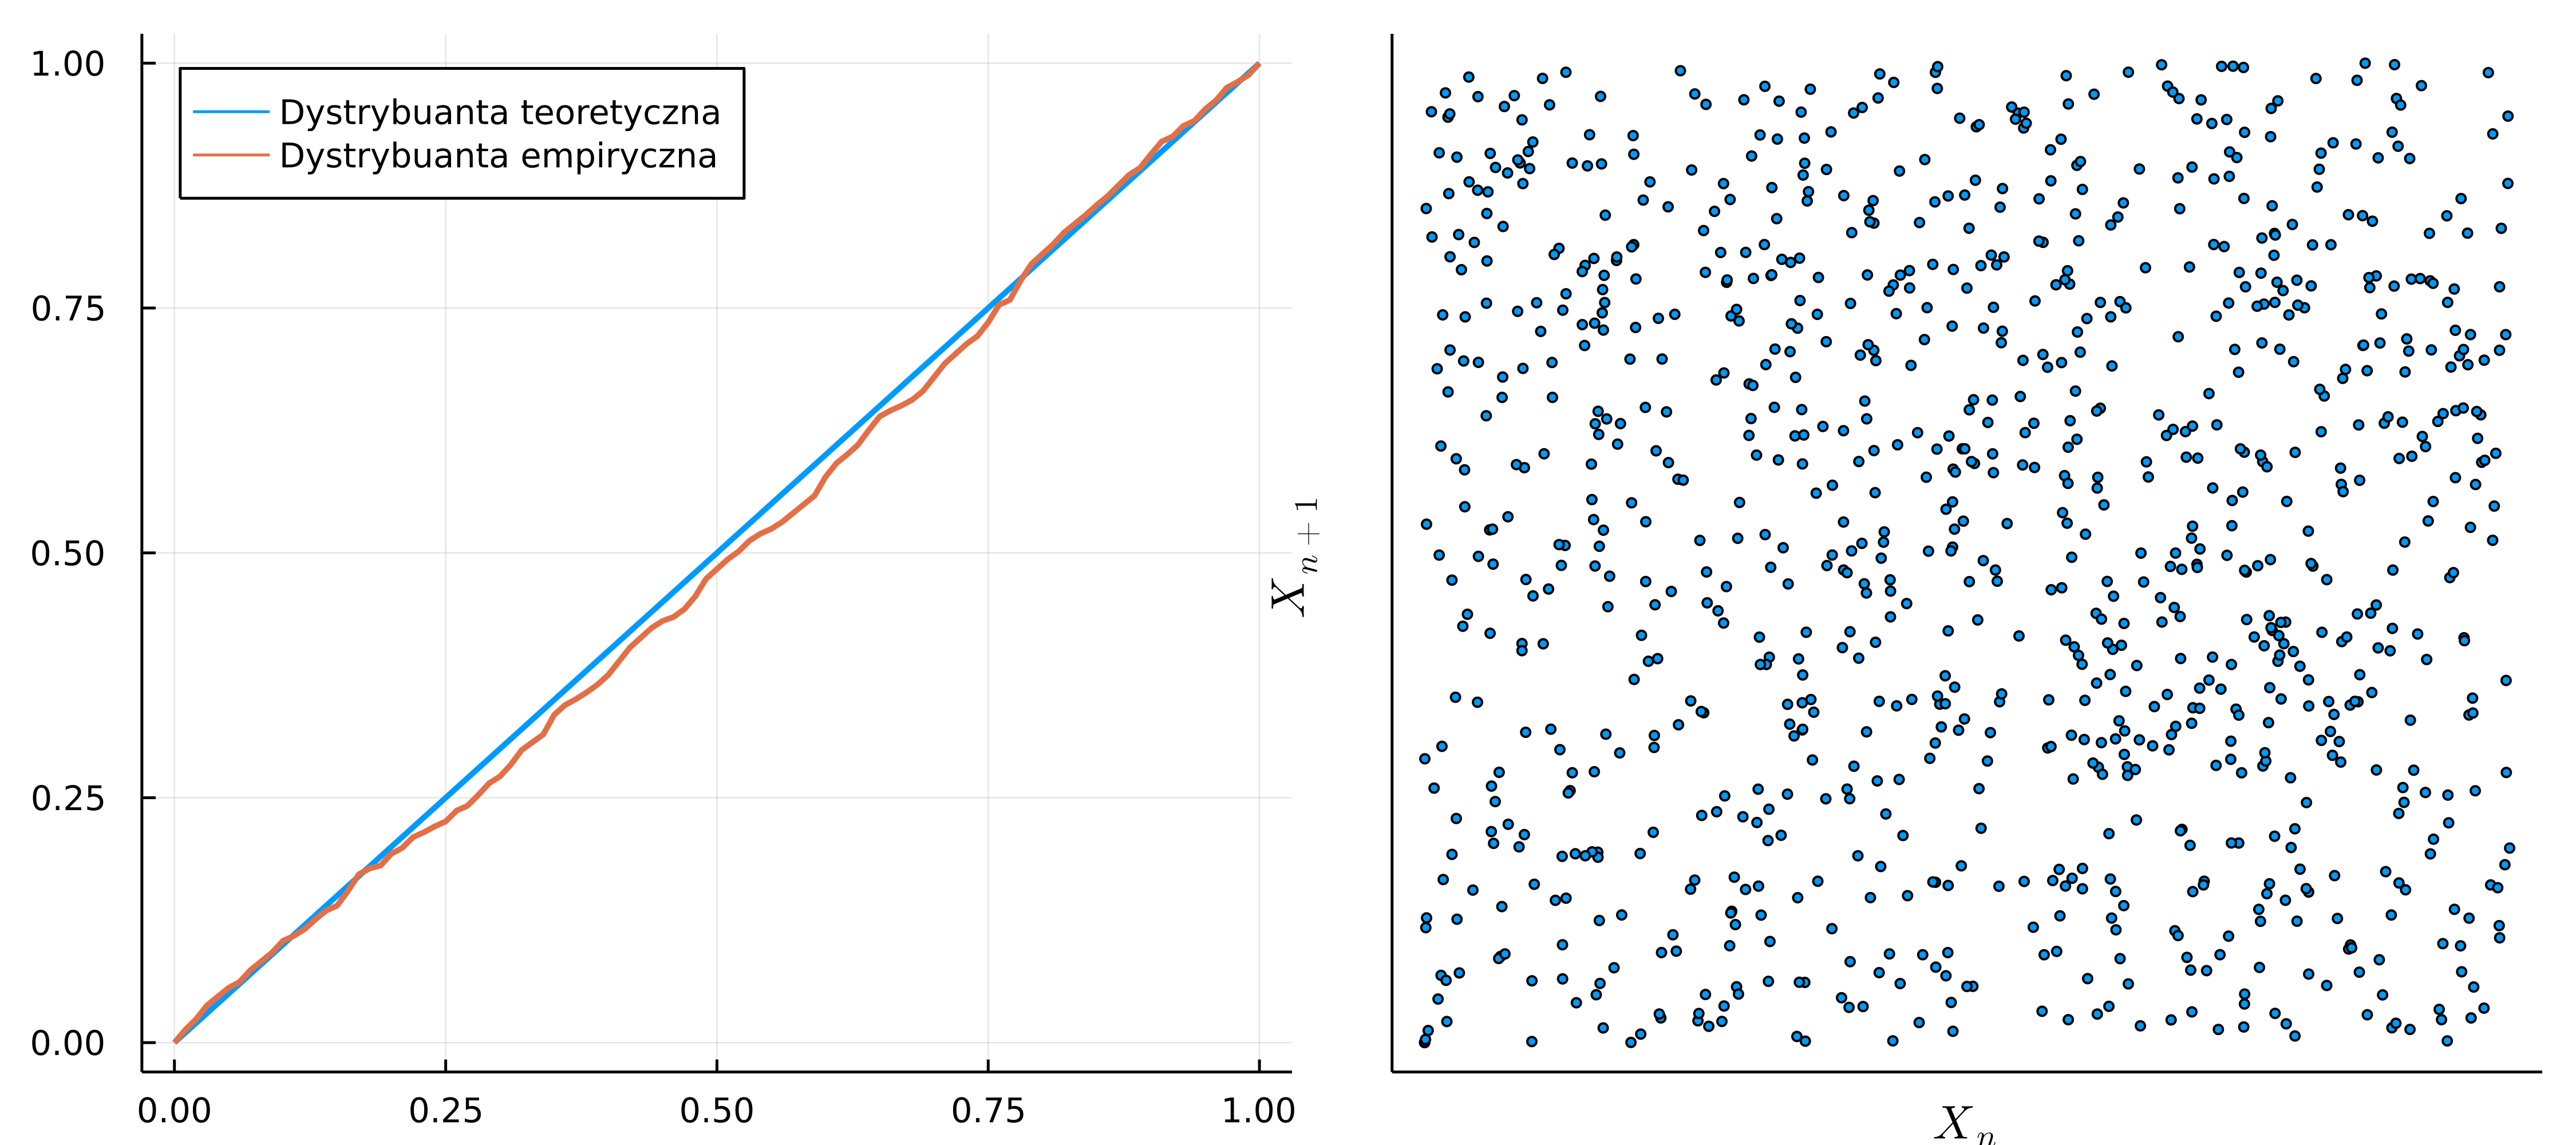
\includegraphics[scale=0.1]{fig/fig_gen1.png}
		\end{figure}
		\begin{figure}[H]
			\centering
			\caption{Test 3D dla 100 000 liczb.}
			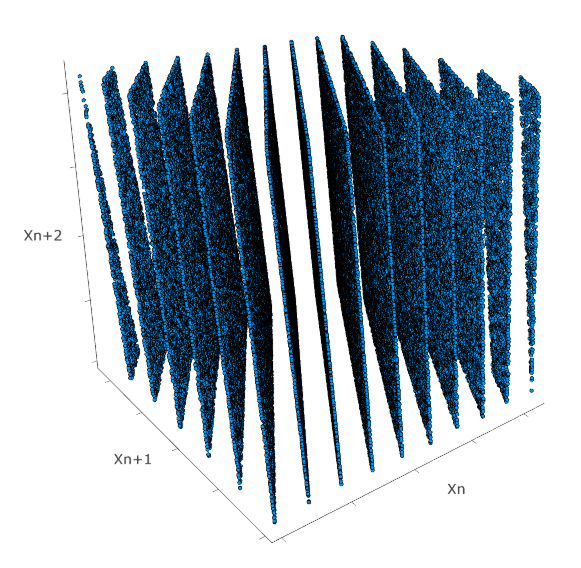
\includegraphics[scale=0.7]{fig/fig_gen2.png}
		\end{figure}
		Widzimy, że dystrybuanta empiryczna pokrywa się z teoretyczną. Z kolei na teście 2D punkty wydają się być rozłożone losowo. Jednakże test 3D udowadnia, że liczby te są wygenerowane na podstawie schematu, ponieważ widać wyraźnie, że punkty układają się w uporządkowany sposób. Wniosek jest taki, że generator ten nie jest najlepszy.
		\vspace{6mm}
		\item \textbf{generator VMS's MTH\$RANDOM}: \ $a = 69069$, \ $c = 5$, \ $m = 2^{32}$\\
		Ponownie wybierzmy $x_0 = 1$ i wykonajmy te same testy.
		\begin{figure}[H]
			\centering
			\caption{Po lewej porównanie dystrybuanty empirycznej z teoretyczną rozkładu jednostajnego $\mathcal{U}(0, 1)$, po prawej test 2D. Oba testy przeprowadzone zostały dla 1000 liczb wygenerowanych generatorem VMS's MTH\$RANDOM.}
			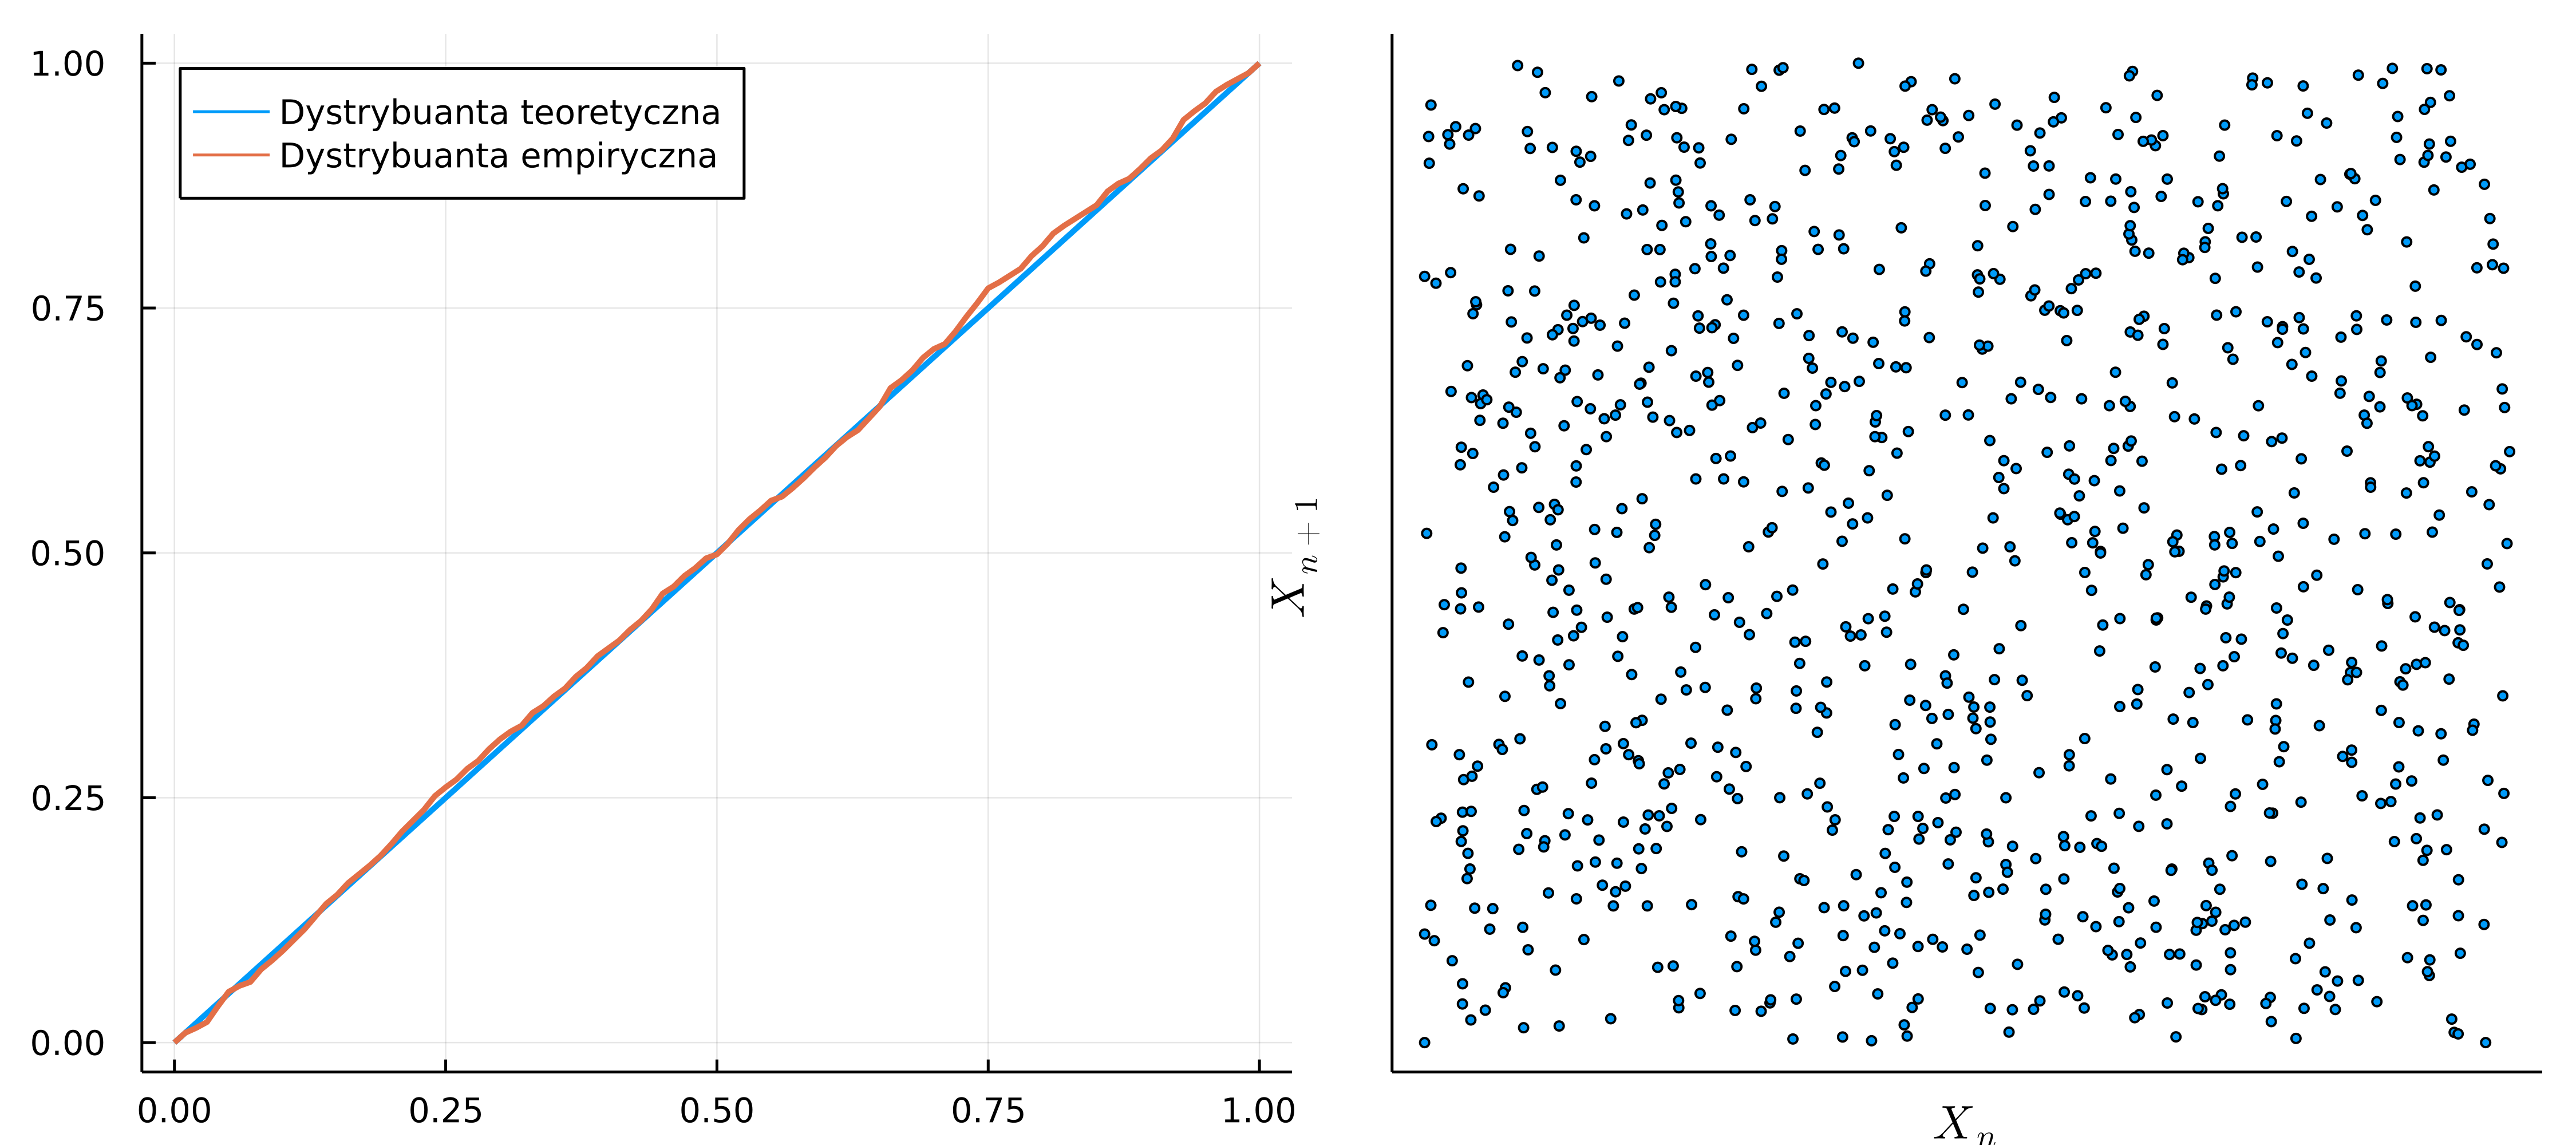
\includegraphics[scale=0.1]{fig/fig_gen3.png}
		\end{figure}
		\begin{figure}[H]
			\centering
			\caption{Test 3D dla 100 000 liczb.}
			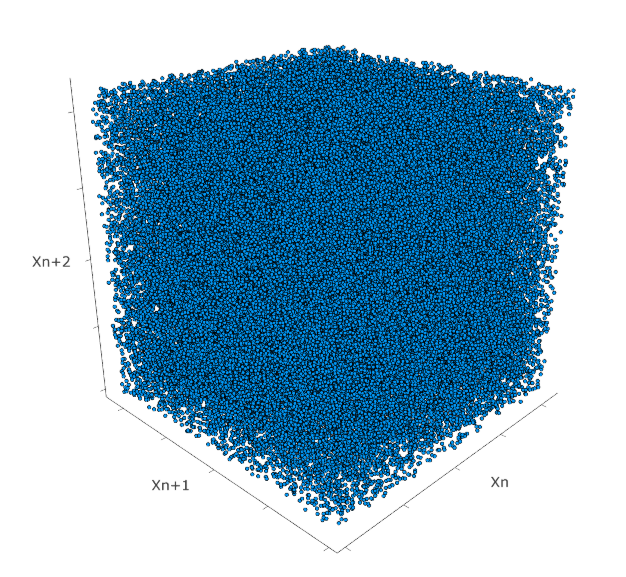
\includegraphics[scale=0.7]{fig/fig_gen4.png}
		\end{figure}
		Jak możemy zauważyć, podobnie jak w poprzednim przykładzie, dystrybuanty empiryczna i teoretyczna są do siebie zbliżone oraz rozłożenie punktów w teście 2D wygląda na losowe. Dodatkowo test 3D także sugeruje niezależne rozłożenie punktów. Na tej podstawie możemy stwierdzić, że generator VMS's MTH\$RANDOM jest zdecydowanie lepszy od generatora RANDU.
	\end{itemize}


%%%%%%%%%%%%%%%%%%%%%%%%%%%%%%%%%%%%%%%%1
	
	\section{Metoda odwrotnej dystrybuanty}
	
	\subsection{Opis}
	\noindent Metoda ta polega na generowaniu zmiennej losowej $X$ generując zmienną $U$ z rozkładu jednostajnego oraz nakładając na nią funkcję odwrotną dystrybuanty.
	\subsubsection{Algorytm dla rozkładów dyskretnych\textsuperscript{\cite{OD - dyskretny}}}
	\noindent Załóżmy, że rozkład $X$ ma postać $\mathrm{P}(X = x_i) = p_\mathrm{i}$, \ $i = 1, 2,\dots $.
	\begin{enumerate}[leftmargin=10mm]
		\item Generuj $U \sim \mathcal{U}(0, 1)$.
		\item Wyznacz $j \in \mathbb{N} $ takie, że $ \sum\limits_{i=1}^{j-1} p_i < U \leqslant \sum\limits_{i=1}^{j} p_i $.
		\item Zwróć $ X = x_i $.
	\end{enumerate}
	\subsubsection{Algorytm dla rozkładów ciągłych\textsuperscript{\cite{OD - dyskretny}}}
	\noindent Załóżmy, że $X$ ma dystrybuantę $F(x)$.
	\begin{enumerate}[leftmargin=10mm]
		\item[a)] Jeśli dystrybuanta jest ściśle rosnąca:
		\begin{enumerate}
			\item[1.] Generuj $U \sim \mathcal{U}(0, 1)$.
			\item[2.] Zwróć $ X = F_X^{-1}(U) $.
		\end{enumerate}
		\vspace{3mm}
		\item[b)] Jeśli dystrybuanta nie jest ściśle rosnąca:
		\begin{enumerate}
			\item[1.] Generuj $U \sim \mathcal{U}(0, 1)$.
			\item[2.] Zwróć $ X = \widetilde{F}_X^{-1}(U) $, gdzie $ \widetilde{F}_X^{-1}(y) = \mathrm{inf}\{x \in \mathbb{R}: F_X(x) \geqslant y\} $.
		\end{enumerate}
	\end{enumerate}

	\subsection{Przykłady}
	
	\subsubsection{Dyskretny - rozkład Poissona}
	\noindent Celem jest wygenerowanie $X \sim \mathcal{P}oiss(\lambda)$, \ $\lambda > 0$. Przypomnijmy jak wygląda rozkład \mbox{Poissona}:
	$$ p_i = \mathrm{P}(X = i) = \mathrm{e}^{-\lambda} \frac{\lambda^i}{i!}. $$
	Zdefiniujmy
	$$ s_j = \sum\limits_{i=0}^{j} p_i. $$
	Algorytm będzie więc polegał na generowaniu $U \sim \mathcal{U}(0, 1)$ i wyznaczaniu $j \in \mathbb{N} $ takiego, że 
	$$ s_{j -1} < U \leqslant s_j. $$
	To znaczy, że musimy sprawdzać kolejne przedziały $(s_{j-1}, s_j)$, czy wpada do nich $U$. W przypadku, gdy $\lambda$, czyli średnia wartość rozkładu zmiennej $X$, jest duża, przechodzenie przez wszystkie przedziały może zajmować sporo czasu. Rozpatrzmy właśnie taki przypadek. Żeby skrócić czas wykonania, możemy zacząć sprawdzanie od przedziału $ (s_{\lceil \lambda \rceil -1}, s_{\lceil \lambda \rceil}) $. Następnie, jeśli $U$ jest mniejsze, to sprawdzamy przedziały na lewo, jeśli większe to na prawo. Dodatkowo zauważmy, że
	$$ p_{i + 1} = p_i \cdot \frac{\lambda}{i + 1}. $$
	Stąd kolejne $p_i$ otrzymamy domnażając $\frac{\lambda}{i + 1}$. Na podstawie tych informacji możemy zbudować algorytm:
	\begin{enumerate}[leftmargin=10mm]
		\item Oblicz wartości $p_i$ oraz $s_i$ dla $i = 0, 1, \dots, \lceil\lambda\rceil$.
		\item Zdefiniuj $j = \lceil \lambda \rceil$, \ $p = p_{\lceil\lambda\rceil}$, \ $F = s_{\lceil\lambda\rceil}$.
		\item Generuj $U \sim \mathcal{U}(0, 1)$.
		\item Jeśli $U > s$:
		\begin{enumerate}[leftmargin=10mm]
			\item $p = p \cdot \frac{\lambda}{j+1}$\\
			$s = s + p$\\
			$j = j + 1$
			\item Jeżeli $U < s$, zwróć $X = j$. W przeciwnym razie wróć do a).
		\end{enumerate}
		\vspace{2mm}
		Jeśli $U < s$:
		\begin{enumerate}[leftmargin=10mm]
			\item $s = s_{j-1}$\\
			$j = j - 1$
			\item Jeżeli $U > s$, zwróć $X = j + 1$. W przeciwnym razie wróć do a).
		\end{enumerate}
	\end{enumerate}
	\begin{figure}[H]
		\centering
		\caption{Porównanie dystrybuanty empirycznej i teoretycznej dla próby z rozkładu $\mathcal{P}oiss(30)$ o długości $n = 1000$.}
		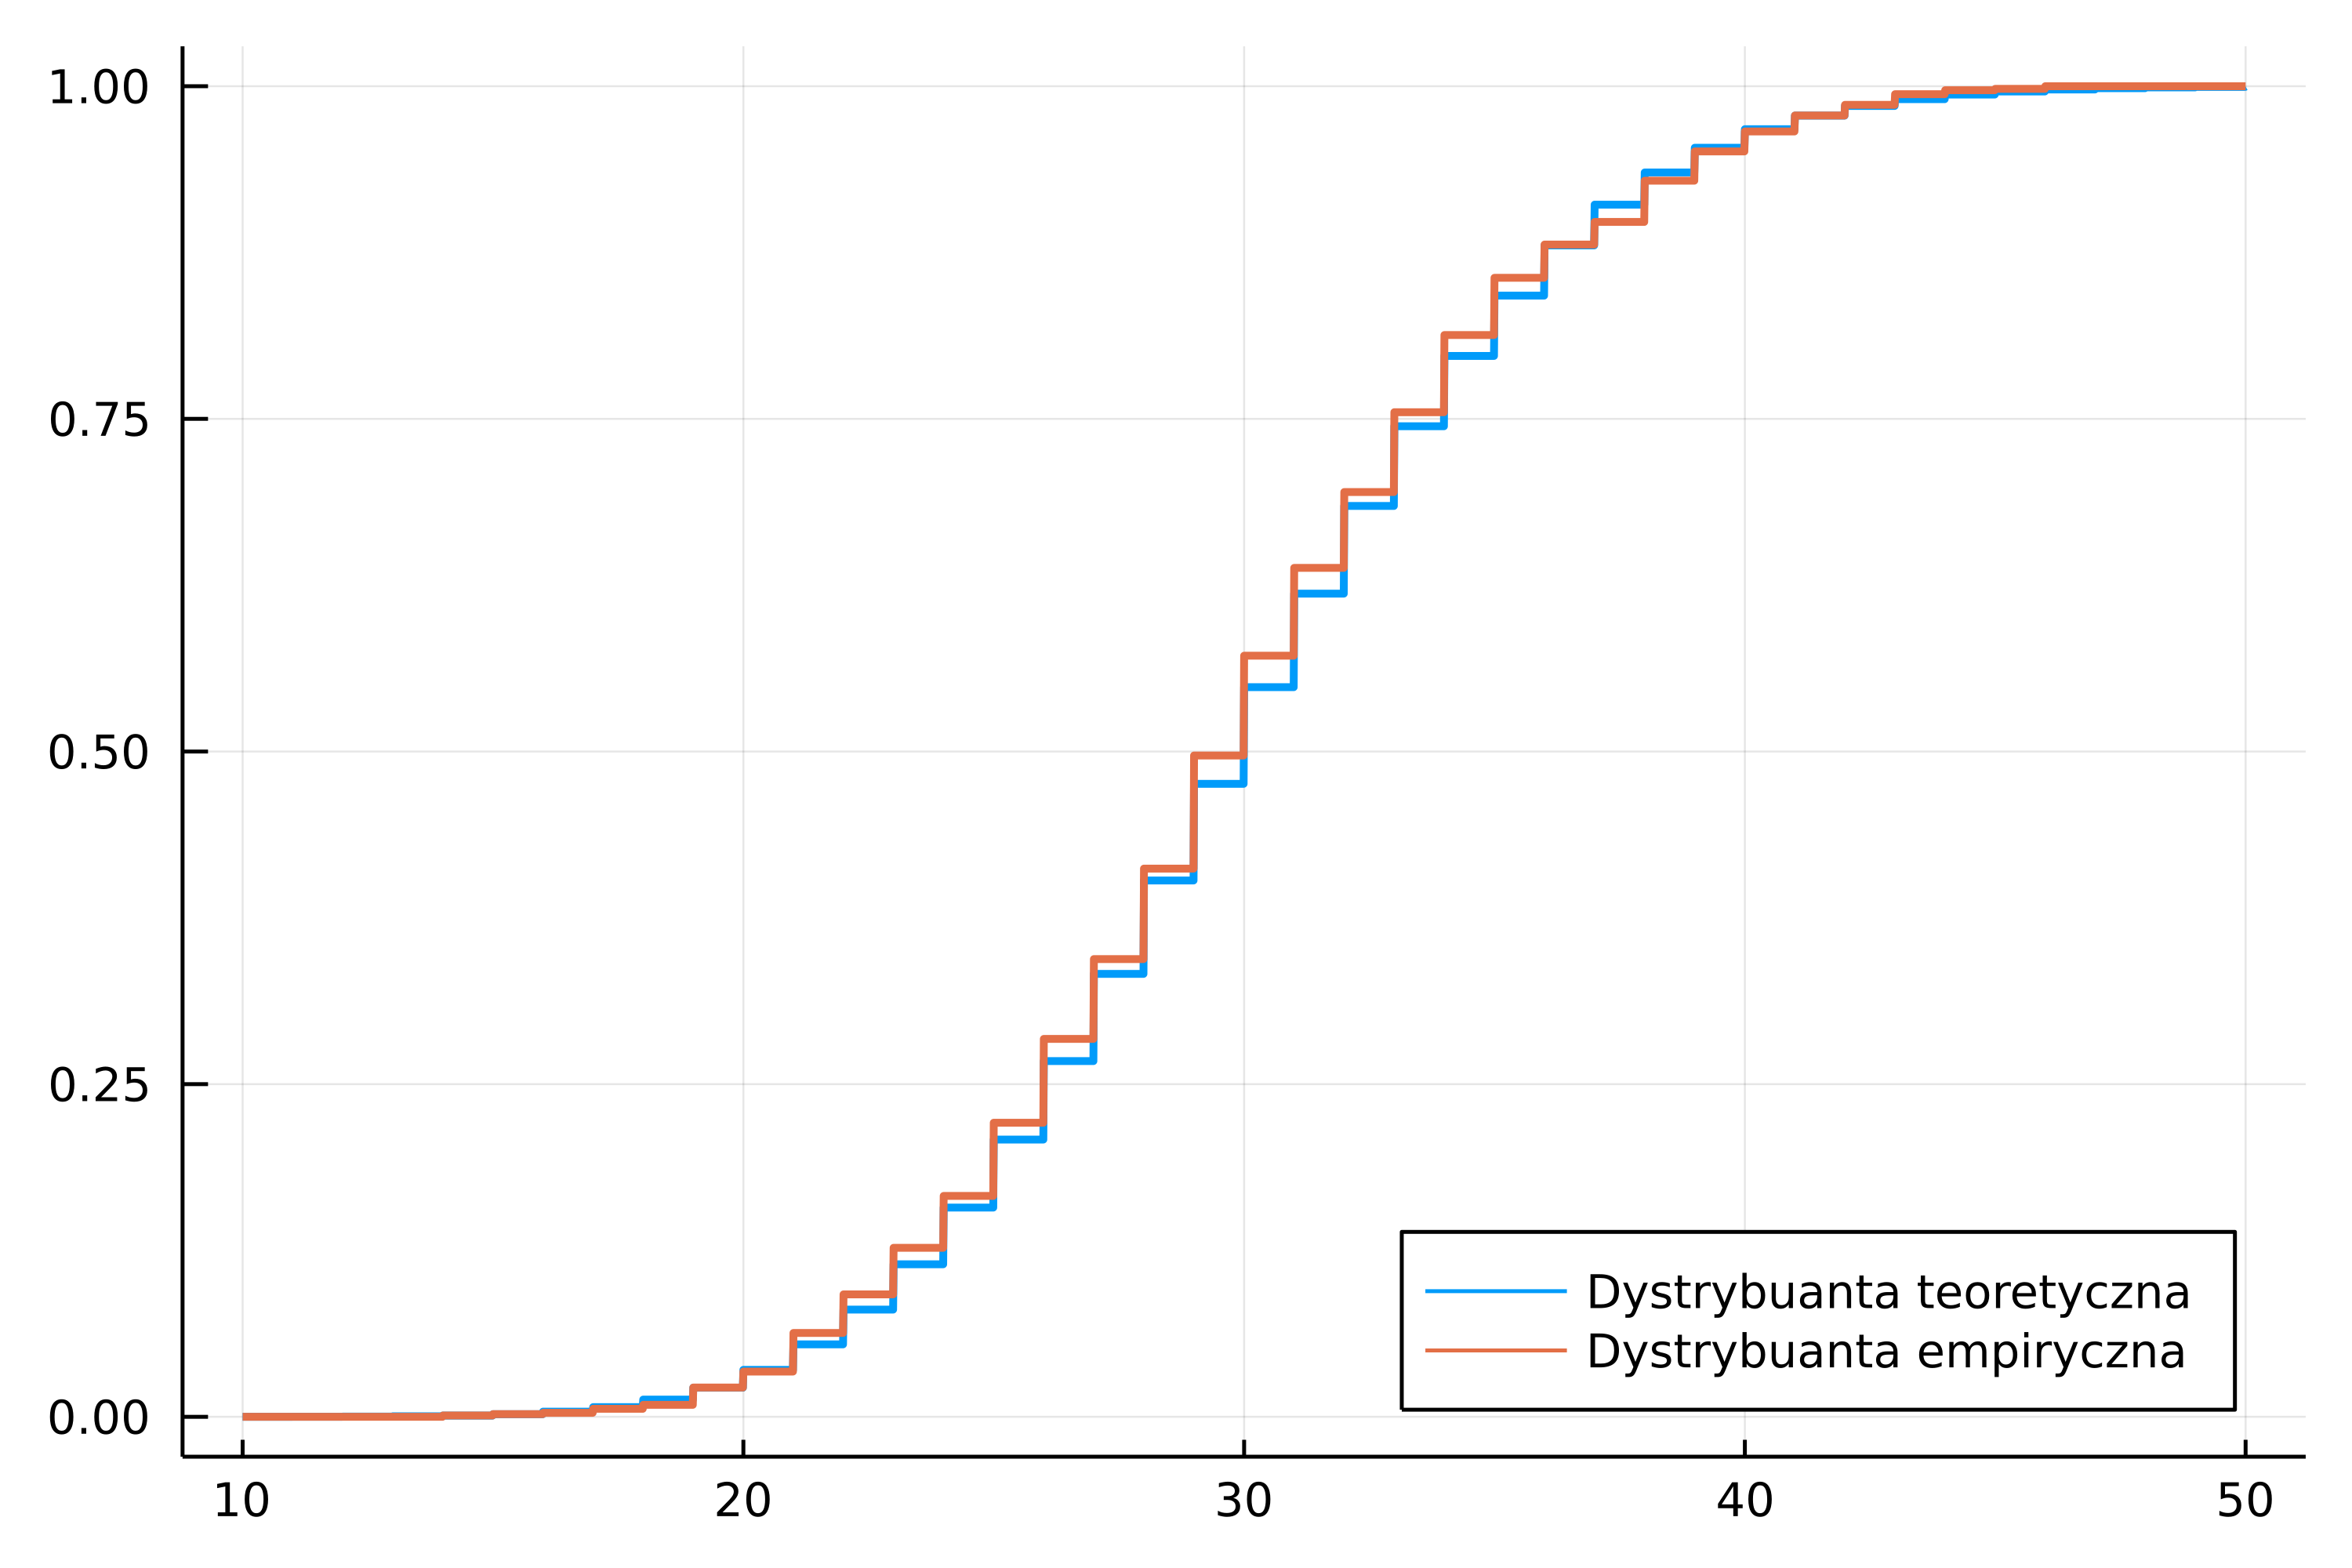
\includegraphics[scale=0.1]{fig/fig_odwr1.png}
	\end{figure}
	
	\subsubsection{Ciągły - rozkład Cauchy'ego}
	\noindent Chcemy wygenerować $ X \sim \mathcal{C}(\mu, \sigma) $. 
	Dystrybuanta rozkładu Cauchy'ego ma postać
	$$ F(x) = \frac{1}{\pi} \arctan{\left(\frac{x - \mu}{\sigma}\right)} + \frac{1}{2}. $$
	Za pomocą elementarnych przekształceń jesteśmy w stanie otrzymać funkcję odwrotną
	$$ F^{-1}(y) = \sigma \tan \left(\pi \left(y - \frac{1}{2}\right) \right) + \mu. $$
	Zatem, żeby wygenerować $X$, należy najpierw wygenerować $U \sim \mathcal{U}(0, 1) $ i zwrócić $F^{-1}(U)$. Możemy to jednak lekko uprościć. Niech $ V \sim \mathcal{U}\left(-\frac{\pi}{2}, \frac{\pi}{2}\right) $. Wtedy
	$$ V \buildrel{d}\over{=} \pi \left(U - \frac{1}{2}\right). $$
	Ostatecznie algorytm będzie wyglądał następująco:
	\begin{enumerate}[leftmargin=10mm]
		\item Generuj $V \sim \mathcal{U}\left(-\frac{\pi}{2}, \frac{\pi}{2}\right)$.
		\item Zwróć $ X = \sigma \tan(V) + \mu $.
	\end{enumerate}
	\begin{figure}[H]
		\centering
		\caption{Porównanie dystrybuanty empirycznej i teoretycznej oraz wykres kwantylowy dla próby z rozkładu $\mathcal{C}(0, 1)$ o długości $n = 1000$.}
		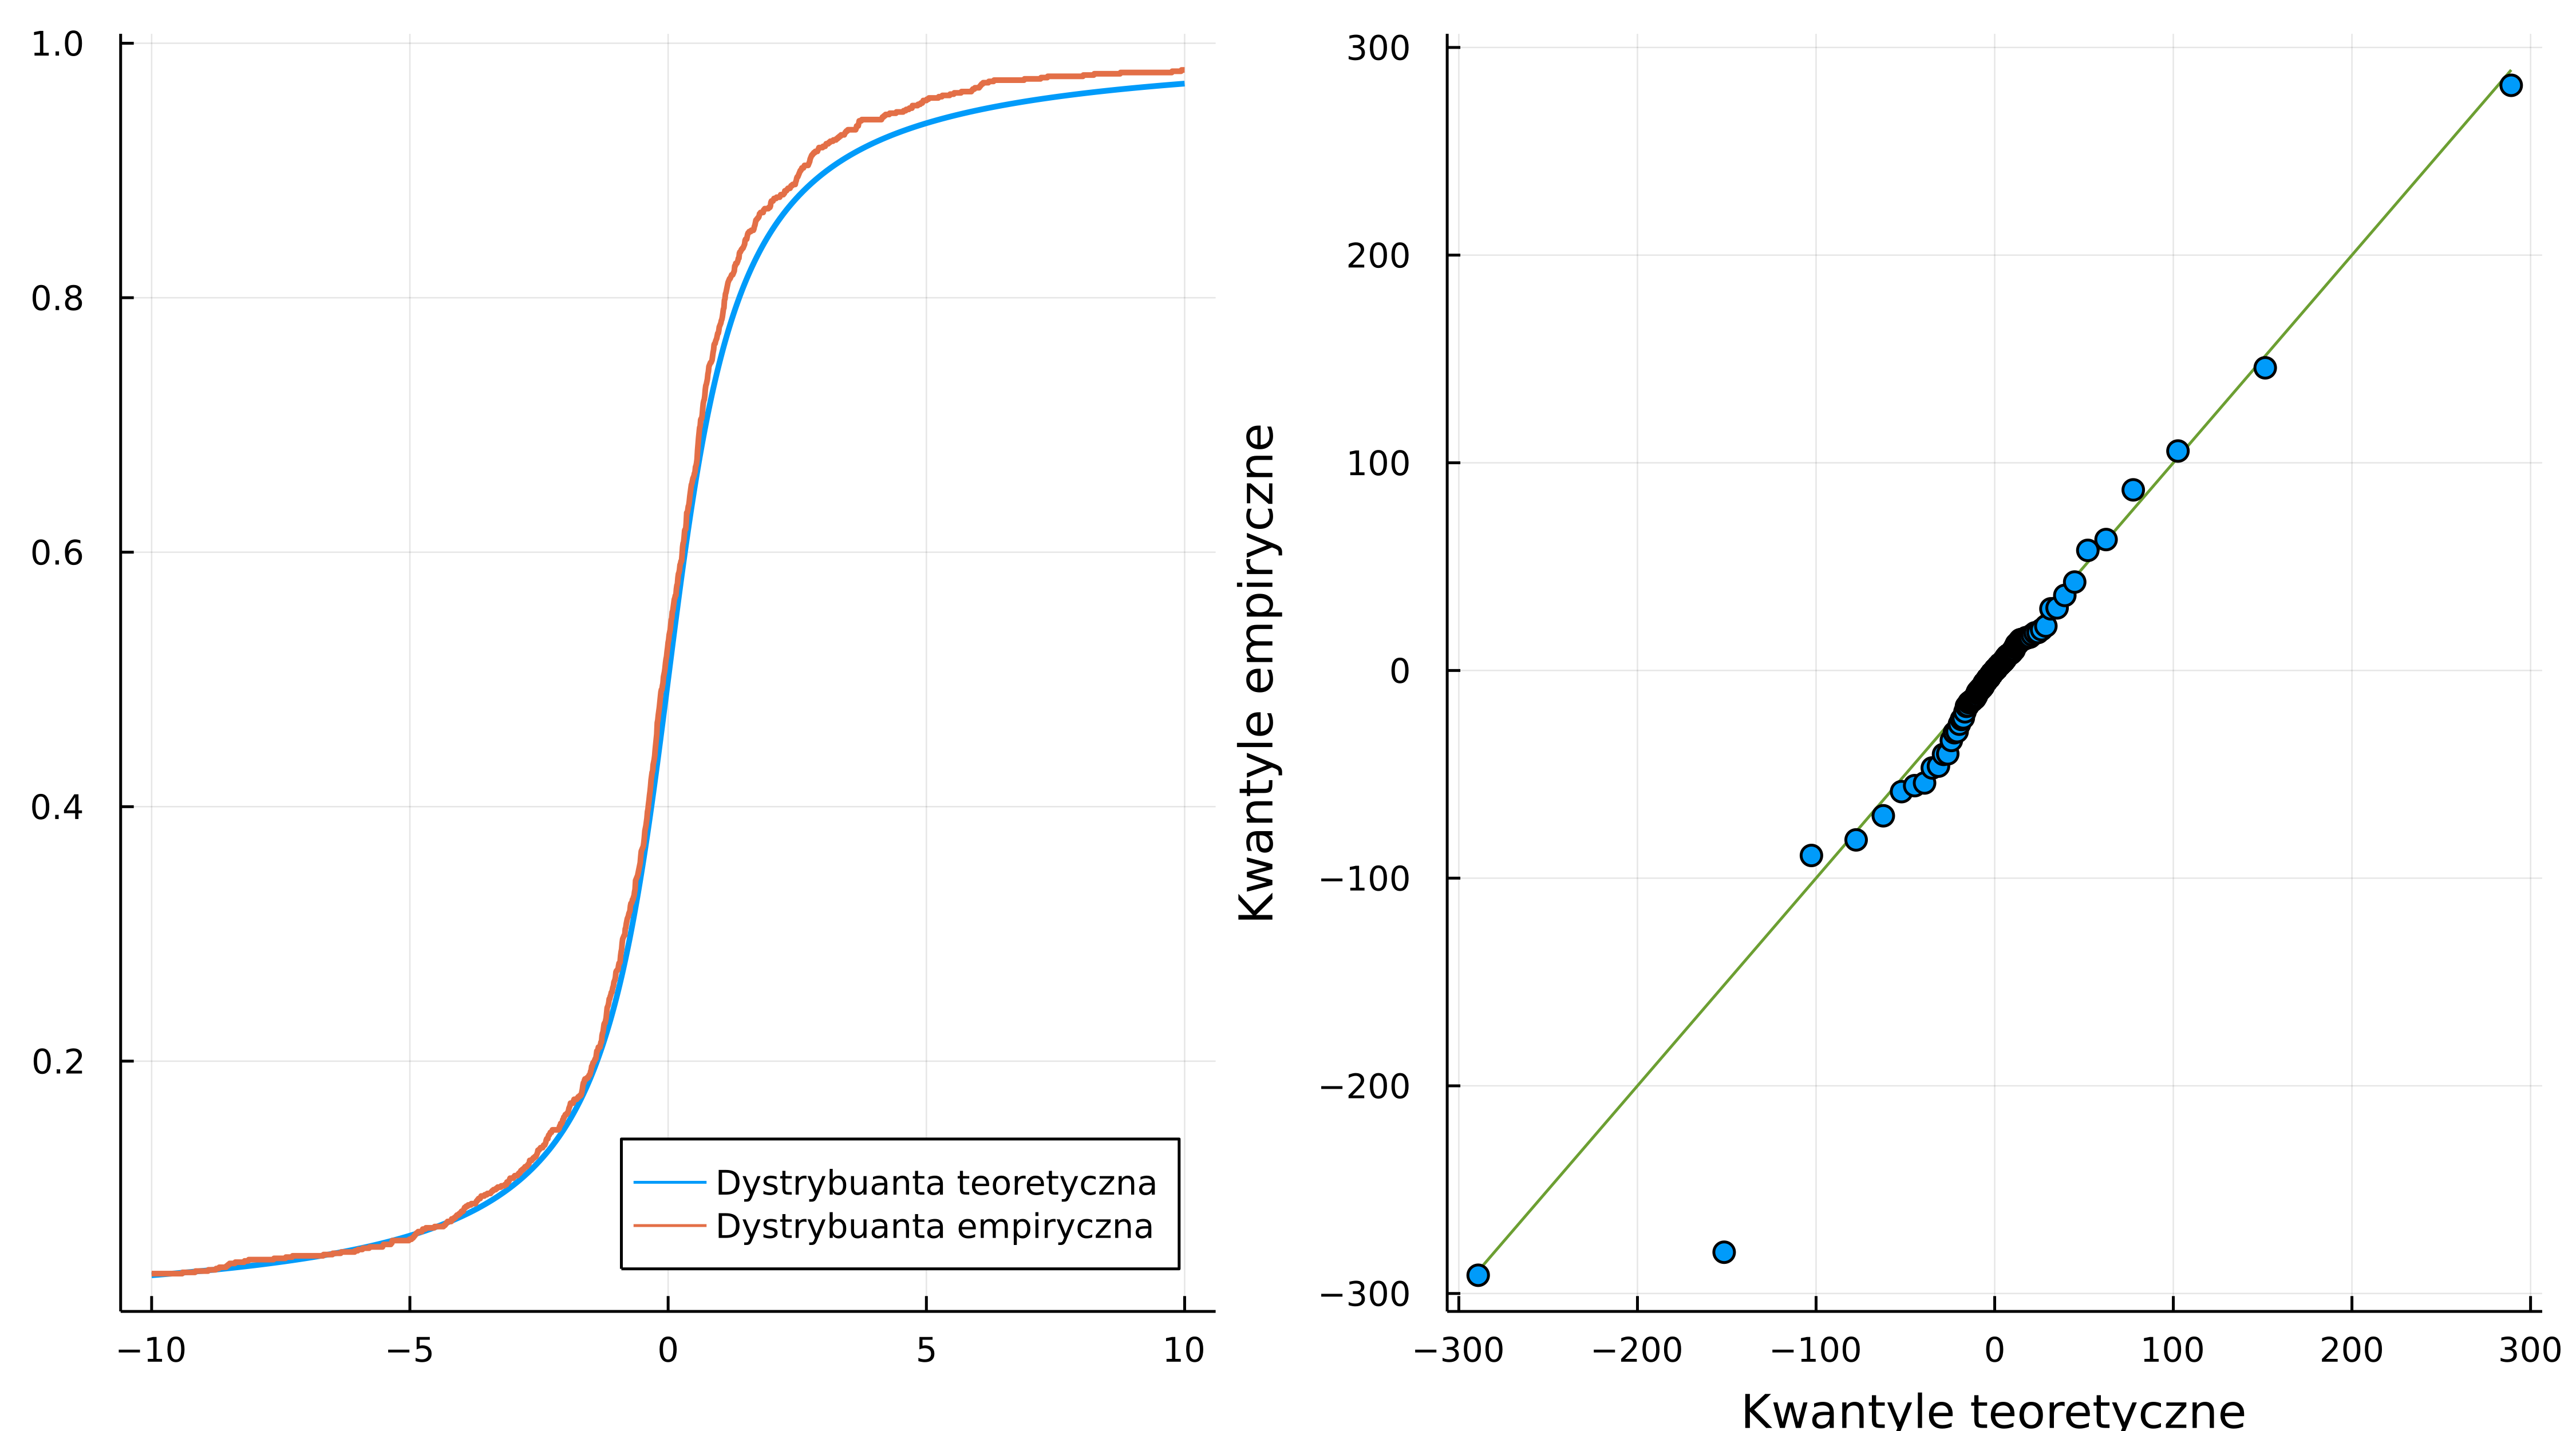
\includegraphics[scale=0.1]{fig/fig_odwr2.png}
	\end{figure}
	%Aby przetestować powyższy algorytm, generujemy wektor 1000 realizacji zmiennej $X$, a następnie porównujemy dystrybuantę empiryczną tej próbki z dystrybuantą teoretyczną oraz tworzymy histogram i porównujemy go z gęstością.
	%Jak możemy zauważyć dystrybuanty empiryczna i teoretyczna są do siebie zbliżone. To samo możemy powiedzieć o krzywej gęstości, której kształt jest podobny do histogramu próby.


%%%%%%%%%%%%%%%%%%%%%%%%%%%%%%%%%%%%%%%%2

	
	\section{Metoda akceptacji i odrzucenia\textsuperscript{\cite{AO - dyskretny}} - Budnik}
	\subsection{Opis metody dla przypadku dyskretnego\textsuperscript{\cite{AO - dyskretny}}}
	\noindent Metoda akceptacji i odrzucenia służy do generowania zmiennej losowej $X$ przy użyciu innych zmiennych. By móc wykorzystać tą metodę muszą być spełnione:
	\begin{itemize}[leftmargin=10mm]
		\item Potrafimy efektywnie generować inną zmienną losową $Y$
		\item Zmienne $X$ oraz $Y$ muszą być skupione na tym samym zbiorze
		\item Potrafimy wyznaczyć stałą $c$ taką że $\dfrac{\mathrm{P}(X=i)}{\mathrm{P}(Y=i)}=\dfrac{p_i}{q_i}\leqslant c$ dla każdego $i$
	\end{itemize}
	Jeśli są spełnione powyższe założenia możemy użyć poniższego algorytmu do generowania zmiennej $X$.
	\subsubsection{Algorytm}
	\begin{enumerate}[leftmargin=10mm]
		\item Generuj jedną realizację $Y$
		\item Generuj $U\sim \mathcal{U}(0,1)$, $U\indep Y$
		\item Jeśli $U\leqslant\frac{p_Y}{cq_Y}$ zwróć $X=Y$, w przeciwnym wróć do 1.
	\end{enumerate}
	
	
	\subsection{Opis metody dla przypadku ciągłego\textsuperscript{\cite{AO - ciagly}}}
	M\noindent etoda akceptacji i odrzucenia służy do generowania zmiennej losowej $X$ o gęstości $f(x)$ przy użyciu innych zmiennych. By móc wykorzystać tą metodę muszą być spełnione:
	\begin{itemize}[leftmargin=10mm]
		\item Potrafimy efektywnie generować inną zmienną losową $Y$ o gęstości $g(x)$
		\item Zmienne $X$ oraz $Y$ muszą być skupione na tym samym zbiorze
		\item Potrafimy wyznaczyć stałą $c$ taką że $\sup\dfrac{f(x)}{g(x)}\leqslant c$ dla każdego $x$, gdzie $g(x)\neq0$ (więc również $f(x)\neq0$)
	\end{itemize}
	\subsubsection{Algorytm}
	\begin{enumerate}[leftmargin=10mm]
		\item Generuj jedną realizację $Y$
		\item Generuj $U\sim \mathcal{U}(0,1)$, $U\indep Y$
		\item Jeśli $U\leqslant\dfrac{f(Y)}{cg(Y)}$ zwróć $X=Y$, w przeciwnym wróć do 1.
	\end{enumerate}

	\subsection{Szybkość algorytmu}
	\noindent W obu przypadkach, ciągłym i dyskretnym, prawdopodobieństwo, że zmienna zostanie zaakceptowana wynosi $\frac{1}{c}$.\\
%	Średnia liczba powtórzeń algorytmu wynosi $c$, zatem stałą tę powinniśmy dobierać jak najmniejszą spełniającą wymagane kryteria.
	Liczba iteracji algorytmu potrzebnych do wygenerowania zmiennej ma rozkład $\mathcal{G}eom(\frac{1}{c})$, zatem średnia liczba iteracji potrzebna do wygenerowania tej zmiennej to $c$. Z tego powodu stałą tą powinniśmy dobrać jak najmniejszą możliwą. Najoptymalniej wybrać $c=\max\frac{p_Y}{q_Y}$ w przypadku dyskretnym oraz $c=\sup\frac{f(x)}{g(x)}$ dla przypadku ciągłego.
%		Prawdopodobieństwo że zmienna zostanie zaakceptowana wynosi
%	$$\mathbb{P}(\text{'wartość zaakceptowana'})=\frac{1}{c}$$
%	zatem by algorytm był wydajny stała $c$ powinna być jak najmniejsza. Średnia liczba powtórzeń algorytmu wynosi $c$.

	\subsection{Przykłady}
	
	\subsubsection{Dyskretny}
	\noindent Niech $X$ ma następujący rozkład
	\begin{equation}
		\mathrm{P}(X=i)=\begin{cases}
			0.1, \quad\text{dla $i=-2$}\\
			0.2, \quad\text{dla $i=-1$}\\
			0.5, \quad\text{dla $i=\phantom{-}0$}\\
			0.2, \quad\text{dla $i=\phantom{-}1$}\\
%			0.1, \phantom{0}\quad\text{dla $i=\phantom{-}1$}
		\end{cases}
	\end{equation}
	Do generowania tej zmiennej potrzebujemy zmienną, która jest skupiona na tym samym zbiorze. Najprostszym pomysłem jest wykorzystanie zmiennej z rozkładu jednostajnego dyskretnego $Y\sim\mathcal{DU}(-2,-1,0,1)$. Prawdopodobieństwo, że $Y$ przyjmie daną wartość stale wynosi $\frac{1}{4}$, zatem łatwo wyliczyć stałą $c=4\max_i\mathrm{P}(X=i)=4\cdot0.5=2$. Znając tą stałą wystarczy zastosować dany algorytm
	\begin{enumerate}[leftmargin=10mm]
		\item Generuj jedną realizację $Y\sim\lfloor4\cdot\mathcal{U}(0,1)\rfloor-2$
		\item Generuj $U\sim \mathcal{U}(0,1)$, $U\indep Y$
		\item Jeśli $U\leqslant2p_Y$ zwróć $X=Y$, w przeciwnym wróć do 1.
	\end{enumerate}
	\begin{figure}[H]\caption{Sprawdzenie poprawności metody Akceptacji-Odrzucenie dla próby o rozmiarze $n=100$}\label{fig:AO_dysk}
		\centering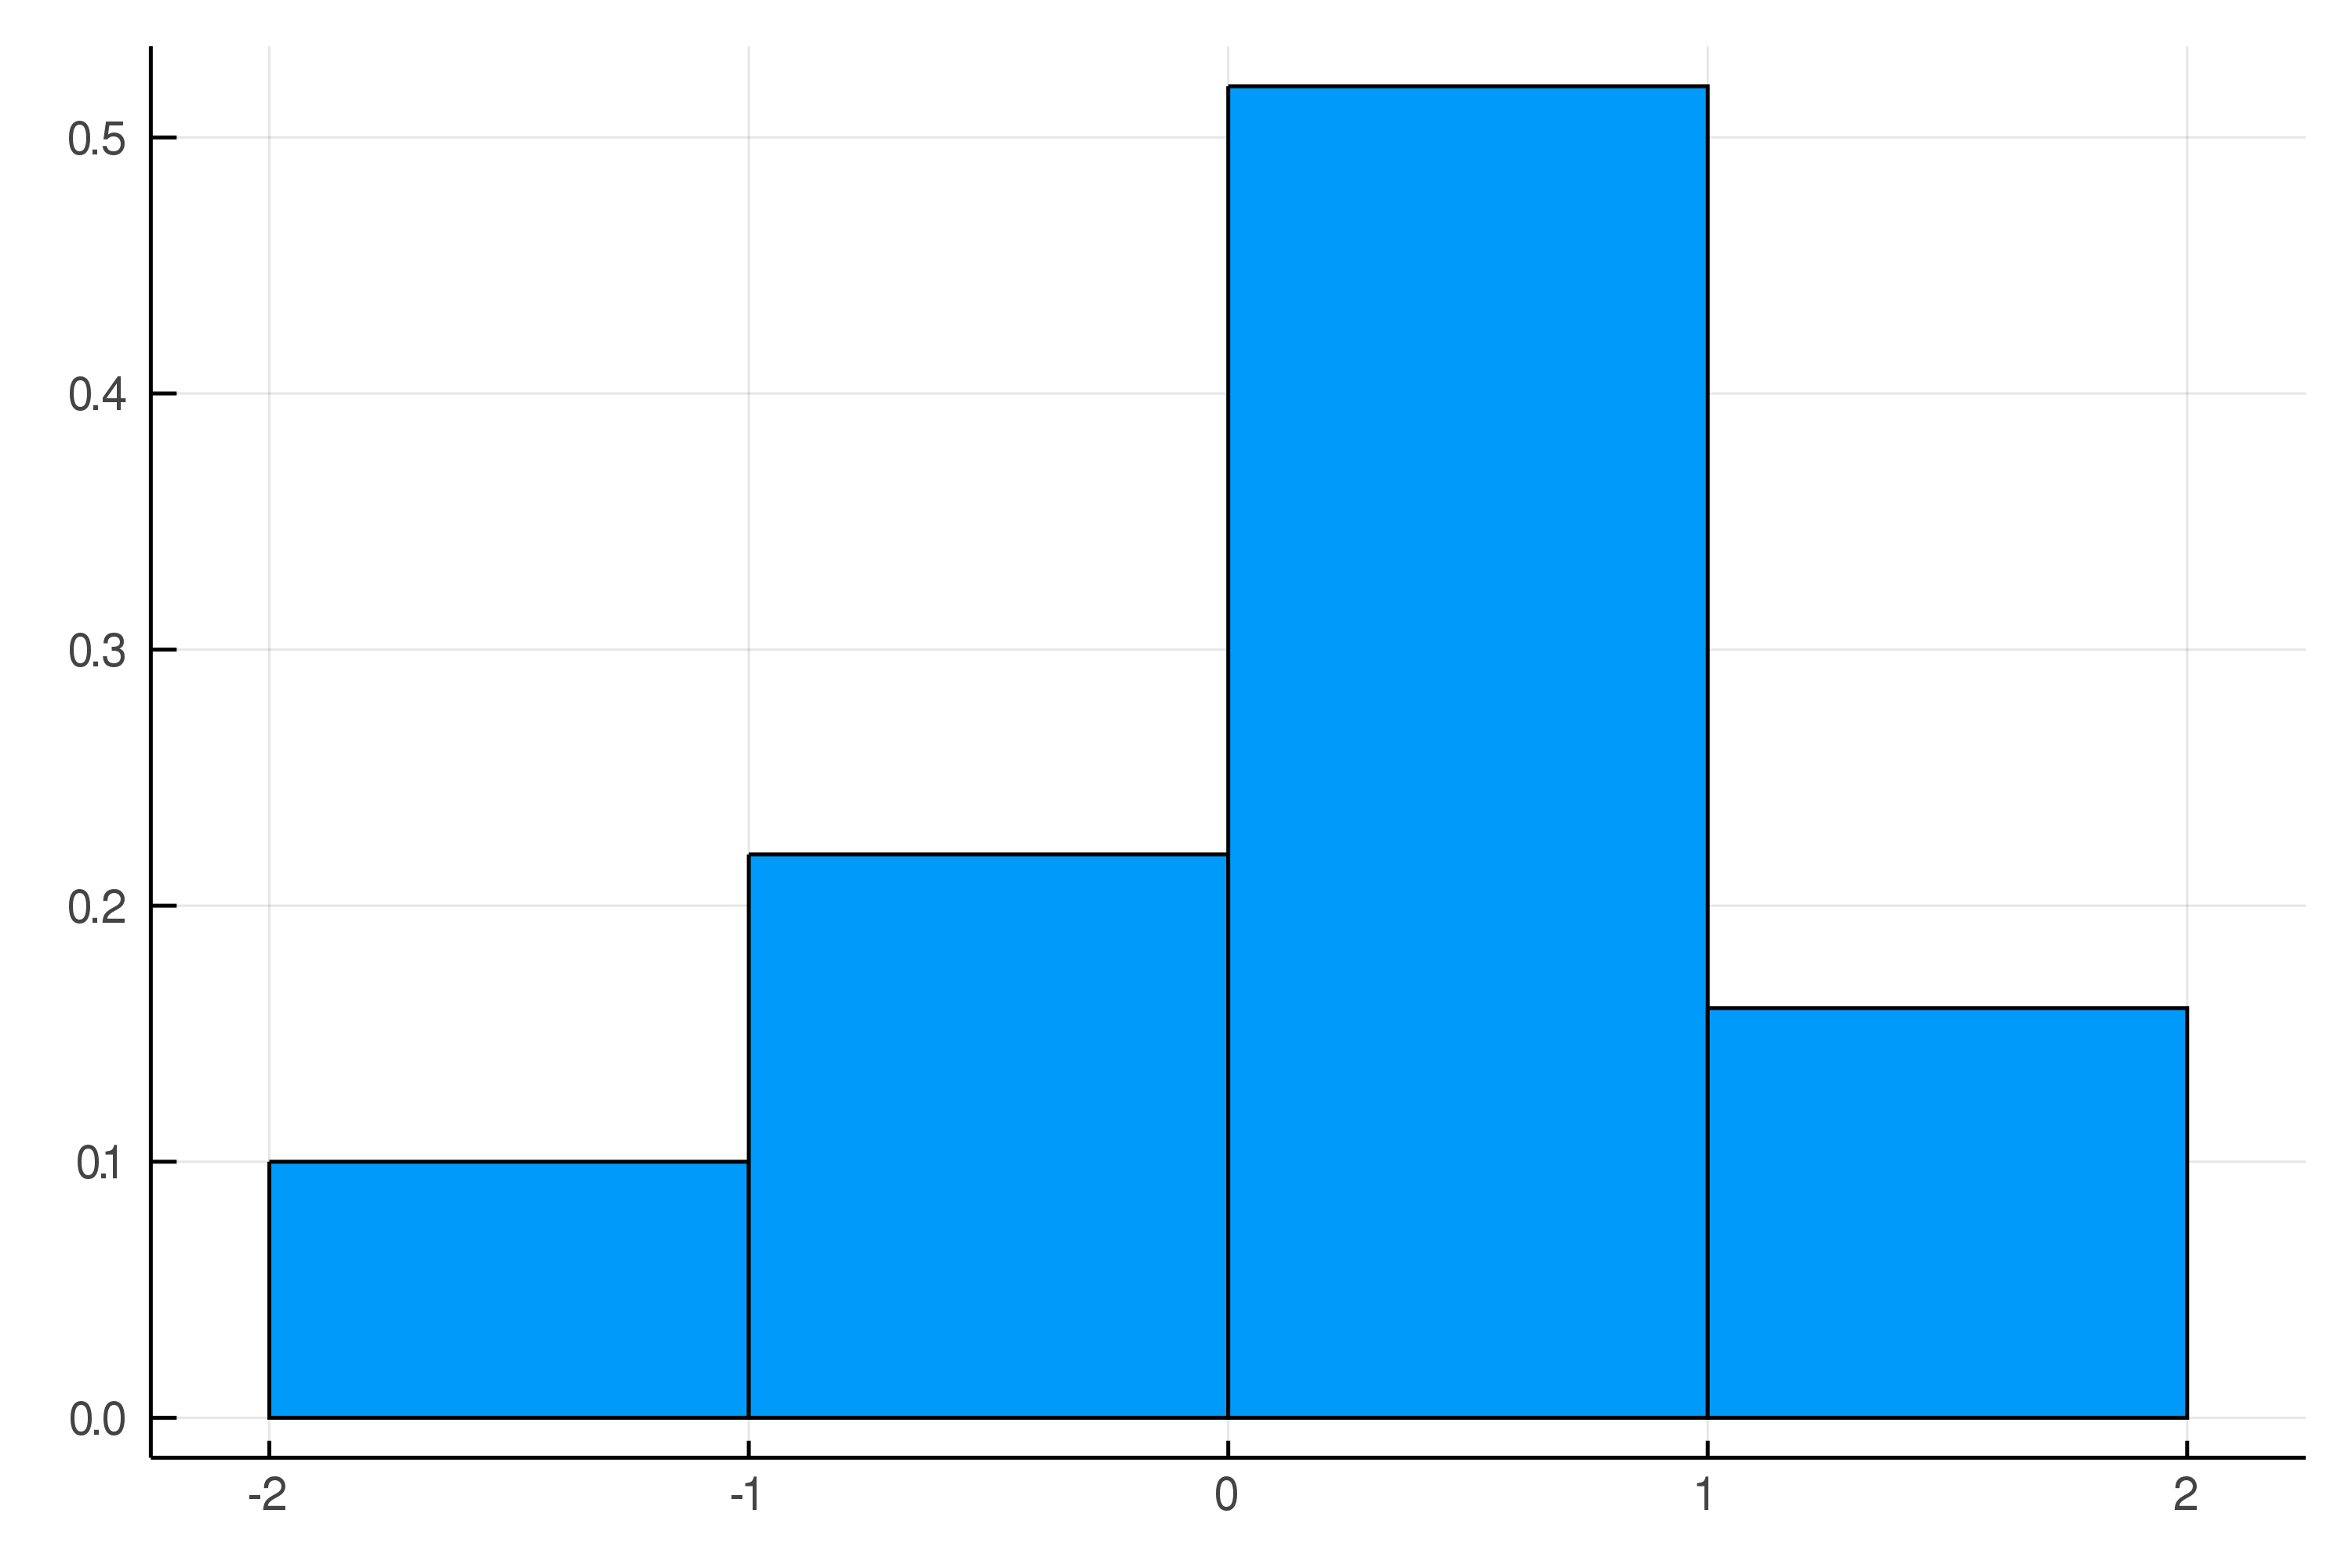
\includegraphics[width=2\columnwidth/3]{fig/fig_AO_dysk.png}
	\end{figure}
	
	
%	Możemy zauważyć, że nasza zmienna ma rozkład skupiony na wym samym zbiorze co $Y=Z-2$, gdzie $Z\sim\mathcal{B}(n=4,p)$. Zmienną $Z$ potrafimy już efektywnie generować przy pomocy metody splotowej. Ale są szybsze sposoby i ten podobny do tego wykonywaliśmy już na zajęciach, ale wszystkie są takie same.
 
 	\subsubsection{Ciągły}
 	\noindent Chcemy wygenerować zmienną $X$ o gęstości $f(x)= \ln(2)\cdot\sin(x)\cdot2^{\cos(x)}\boldmath 1_{(0,\frac{\pi}{2})}$. Użyjemy do tego zmiennej $Y\sim\mathcal{U}(0,\frac{\pi}{2})$ o funkcji gęstości $g(x)=\frac{2}{\pi}\boldmath 1_{(0,\frac{\pi}{2})}$. Zaczniemy od wyliczenia stałej~$c$.
 	\begin{equation}
 		c=\sup\limits_{x\in(0,\frac{\pi}{2})}\frac{f(x)}{g(x)}=\sup\limits_{x\in(0,\frac{\pi}{2})}\sin(x)\cdot2^{\cos(x)}\cdot\frac{\pi\ln(2)}{2}\approx \frac{4}{3}
 	\end{equation}
 	Teraz wystarczy się stosować do następującego algorytmu, czyli
	\begin{enumerate}[leftmargin=10mm]
		\item Generuj $Y\sim \frac{\pi}{2}\mathcal{U}(0,1)$
		\item Generuj $U\sim \mathcal{U}(0,1)$, $U\indep Y$
		\item Jeśli $U\leqslant\sin(Y)\cdot2^{\cos(Y)}\cdot\dfrac{3\pi\ln(2)}{8}$ zwróć $X=Y$, w przeciwnym wróć do 1.
	\end{enumerate}	
%	Stosując się do powyższego algorytmu wygenerowaliśmy próbę rozmiaru $n=10^6$. By sprawdzić, czy nasza metoda jest poprawna na poniższych wykresach porównaliśmy gęstość rozkładu z histogramem wygenerowanej próby oraz dystrybuanty: empiryczną z teoretyczną. 
 	

	\begin{figure}[H]\caption{Sprawdzenie poprawności metody Akceptacji-Odrzucenie dla próby o rozmiarze $n=1000$}\label{fig:AO_con}
		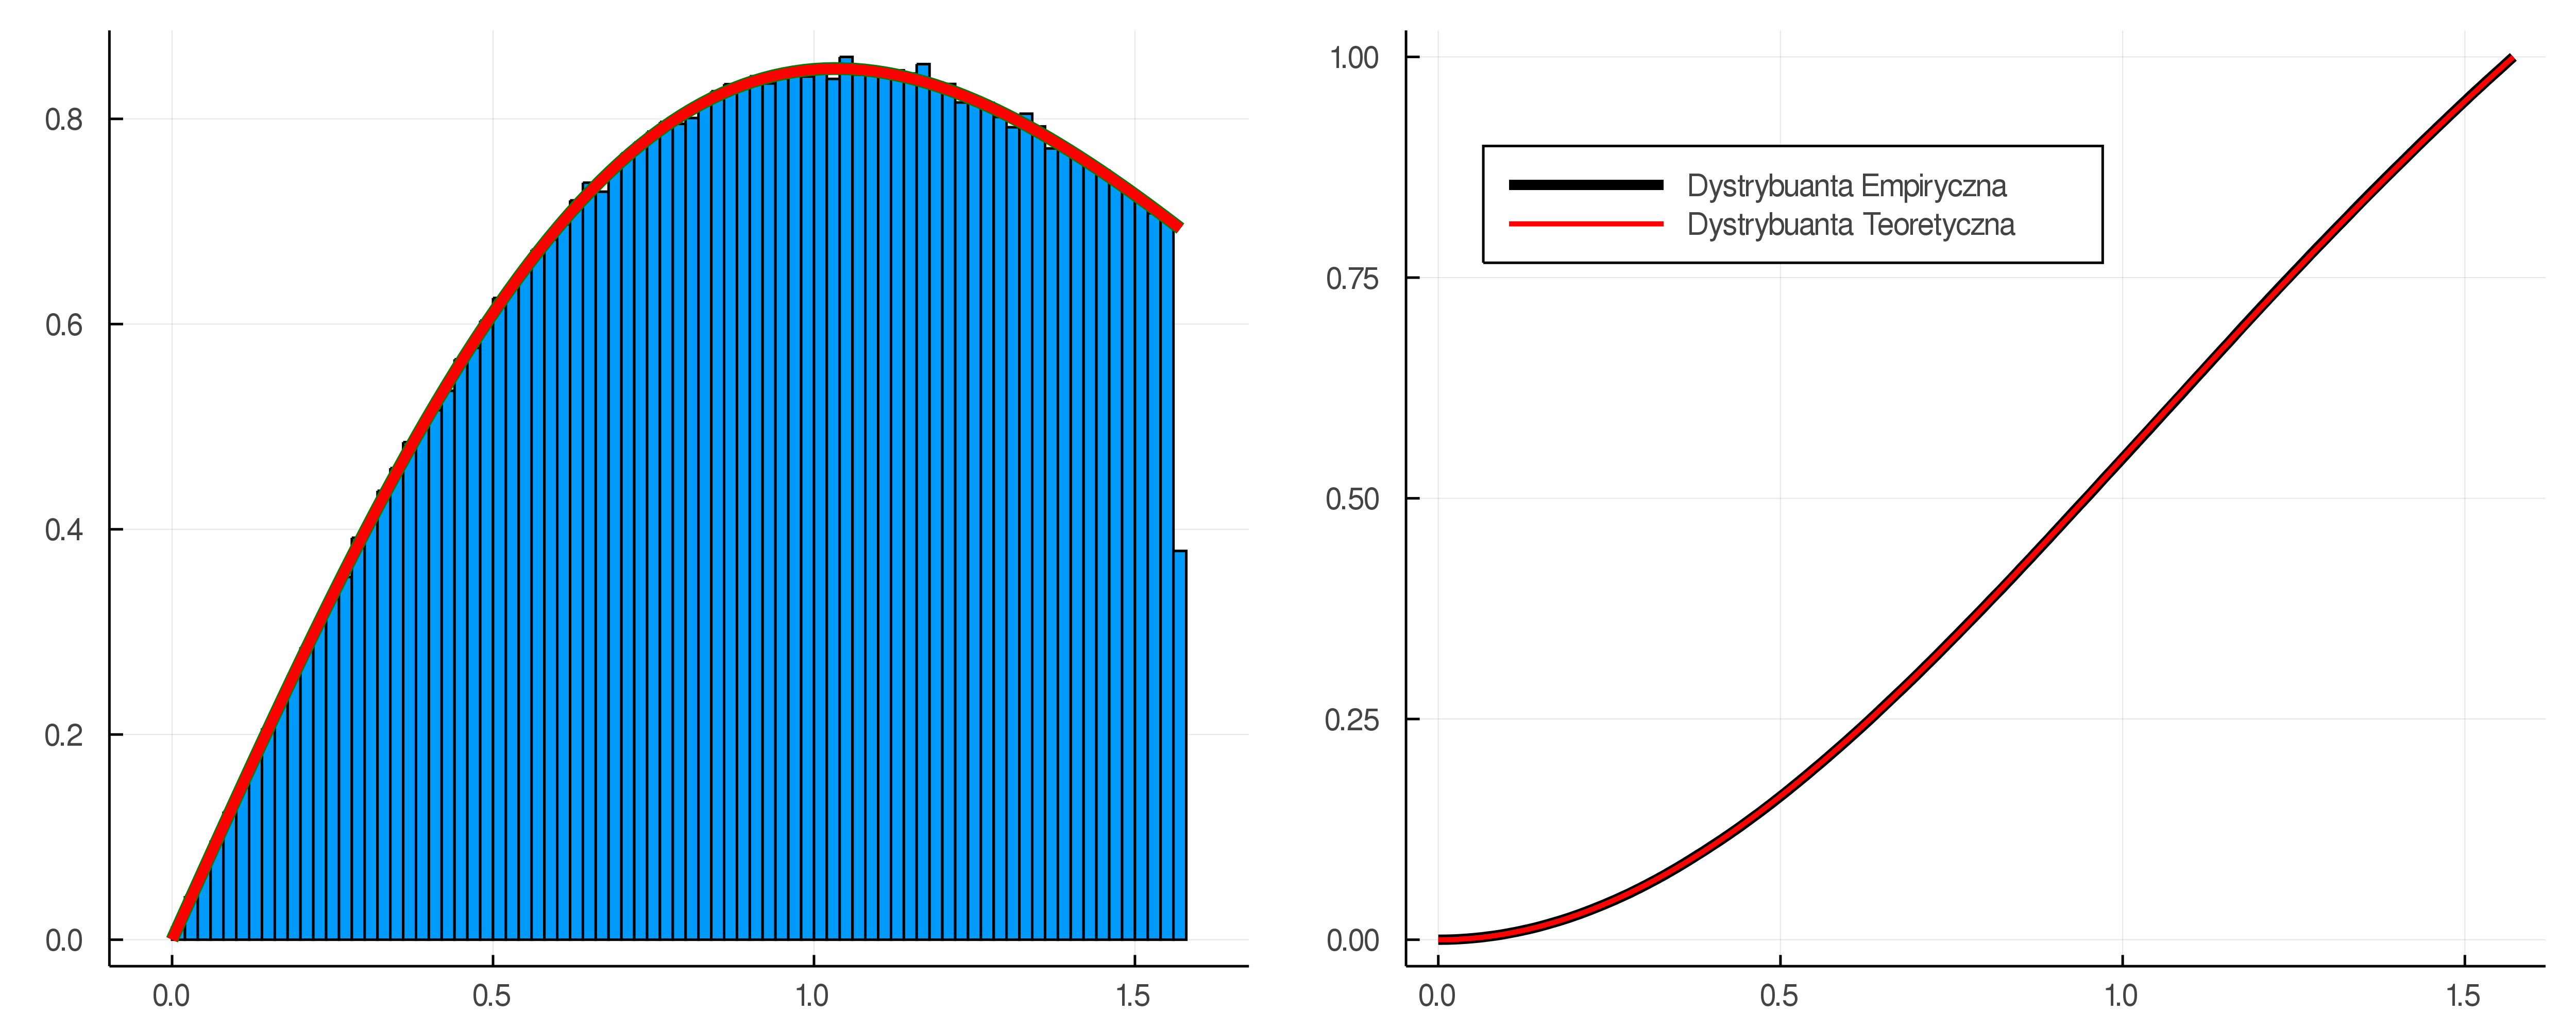
\includegraphics[width=\columnwidth]{fig/fig_AO_con.png}
	\end{figure}
	
%	\begin{figure}[H]\caption{Porównanie na wykresach wygenerowanej }
%		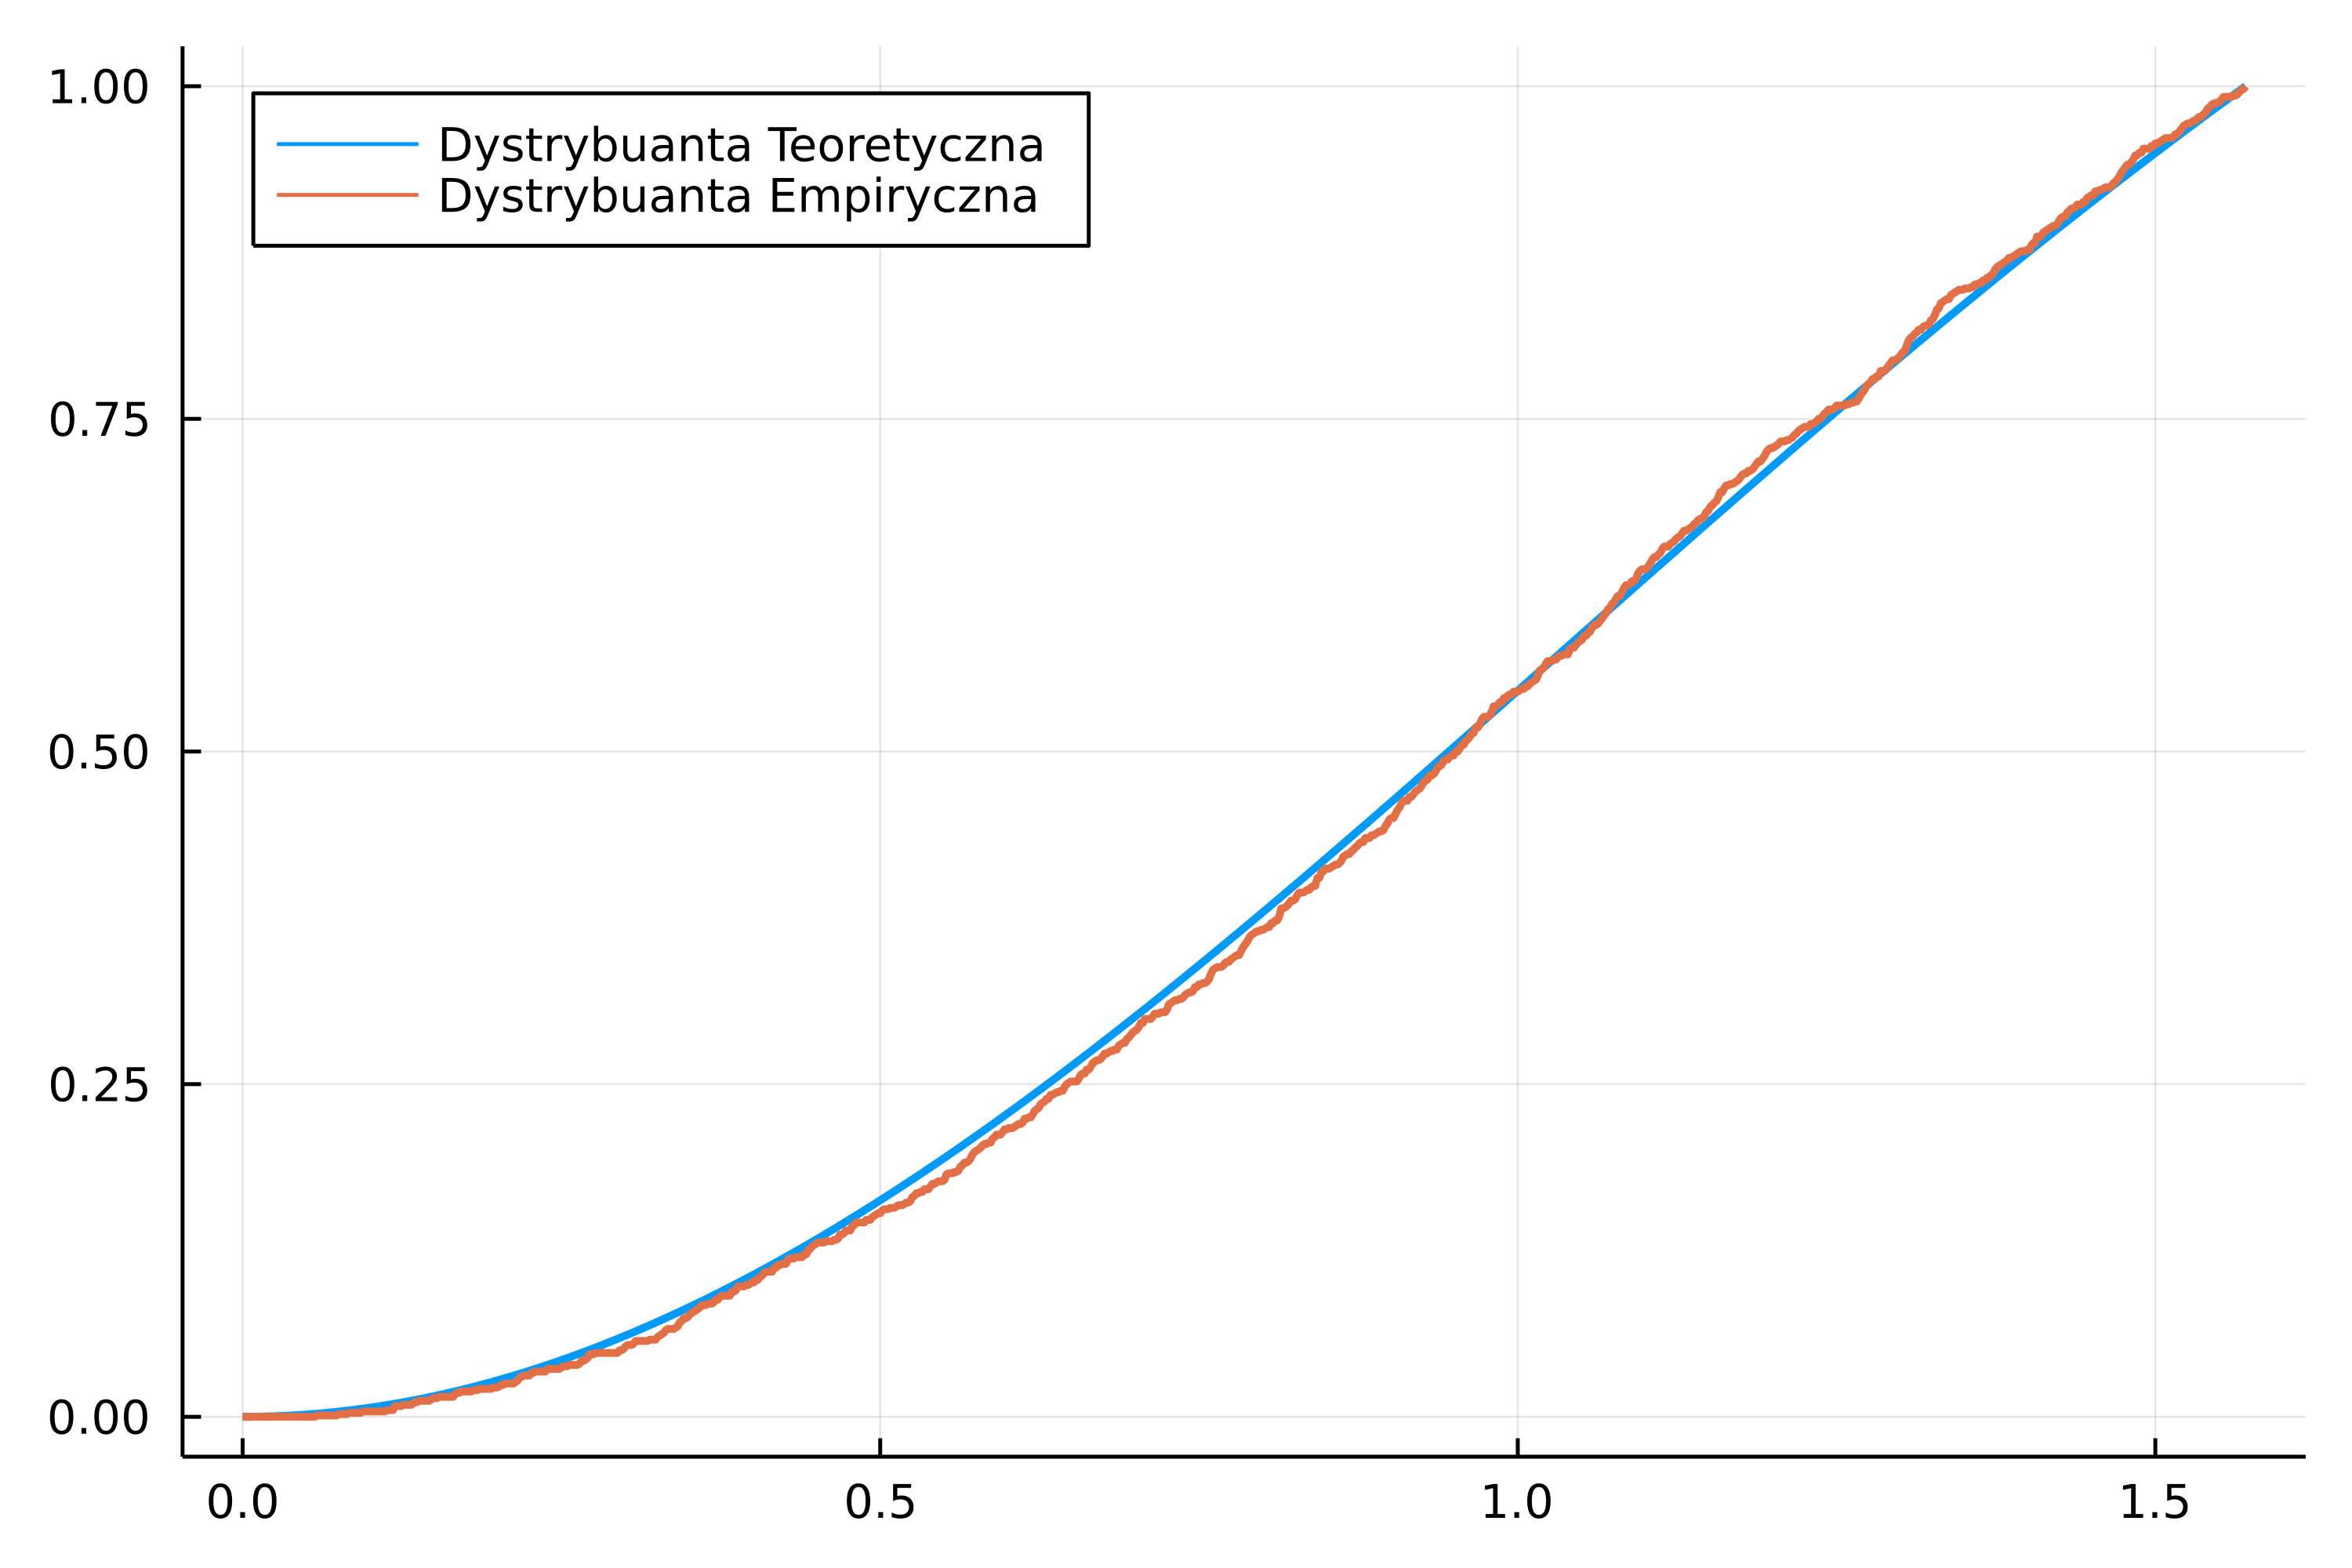
\includegraphics[width=\columnwidth]{fig/fig_AO_con_cdf.png}
%	\end{figure}
%
%	\begin{figure}[H]
%		\centering
%		\subfloat[\centering label 1]{{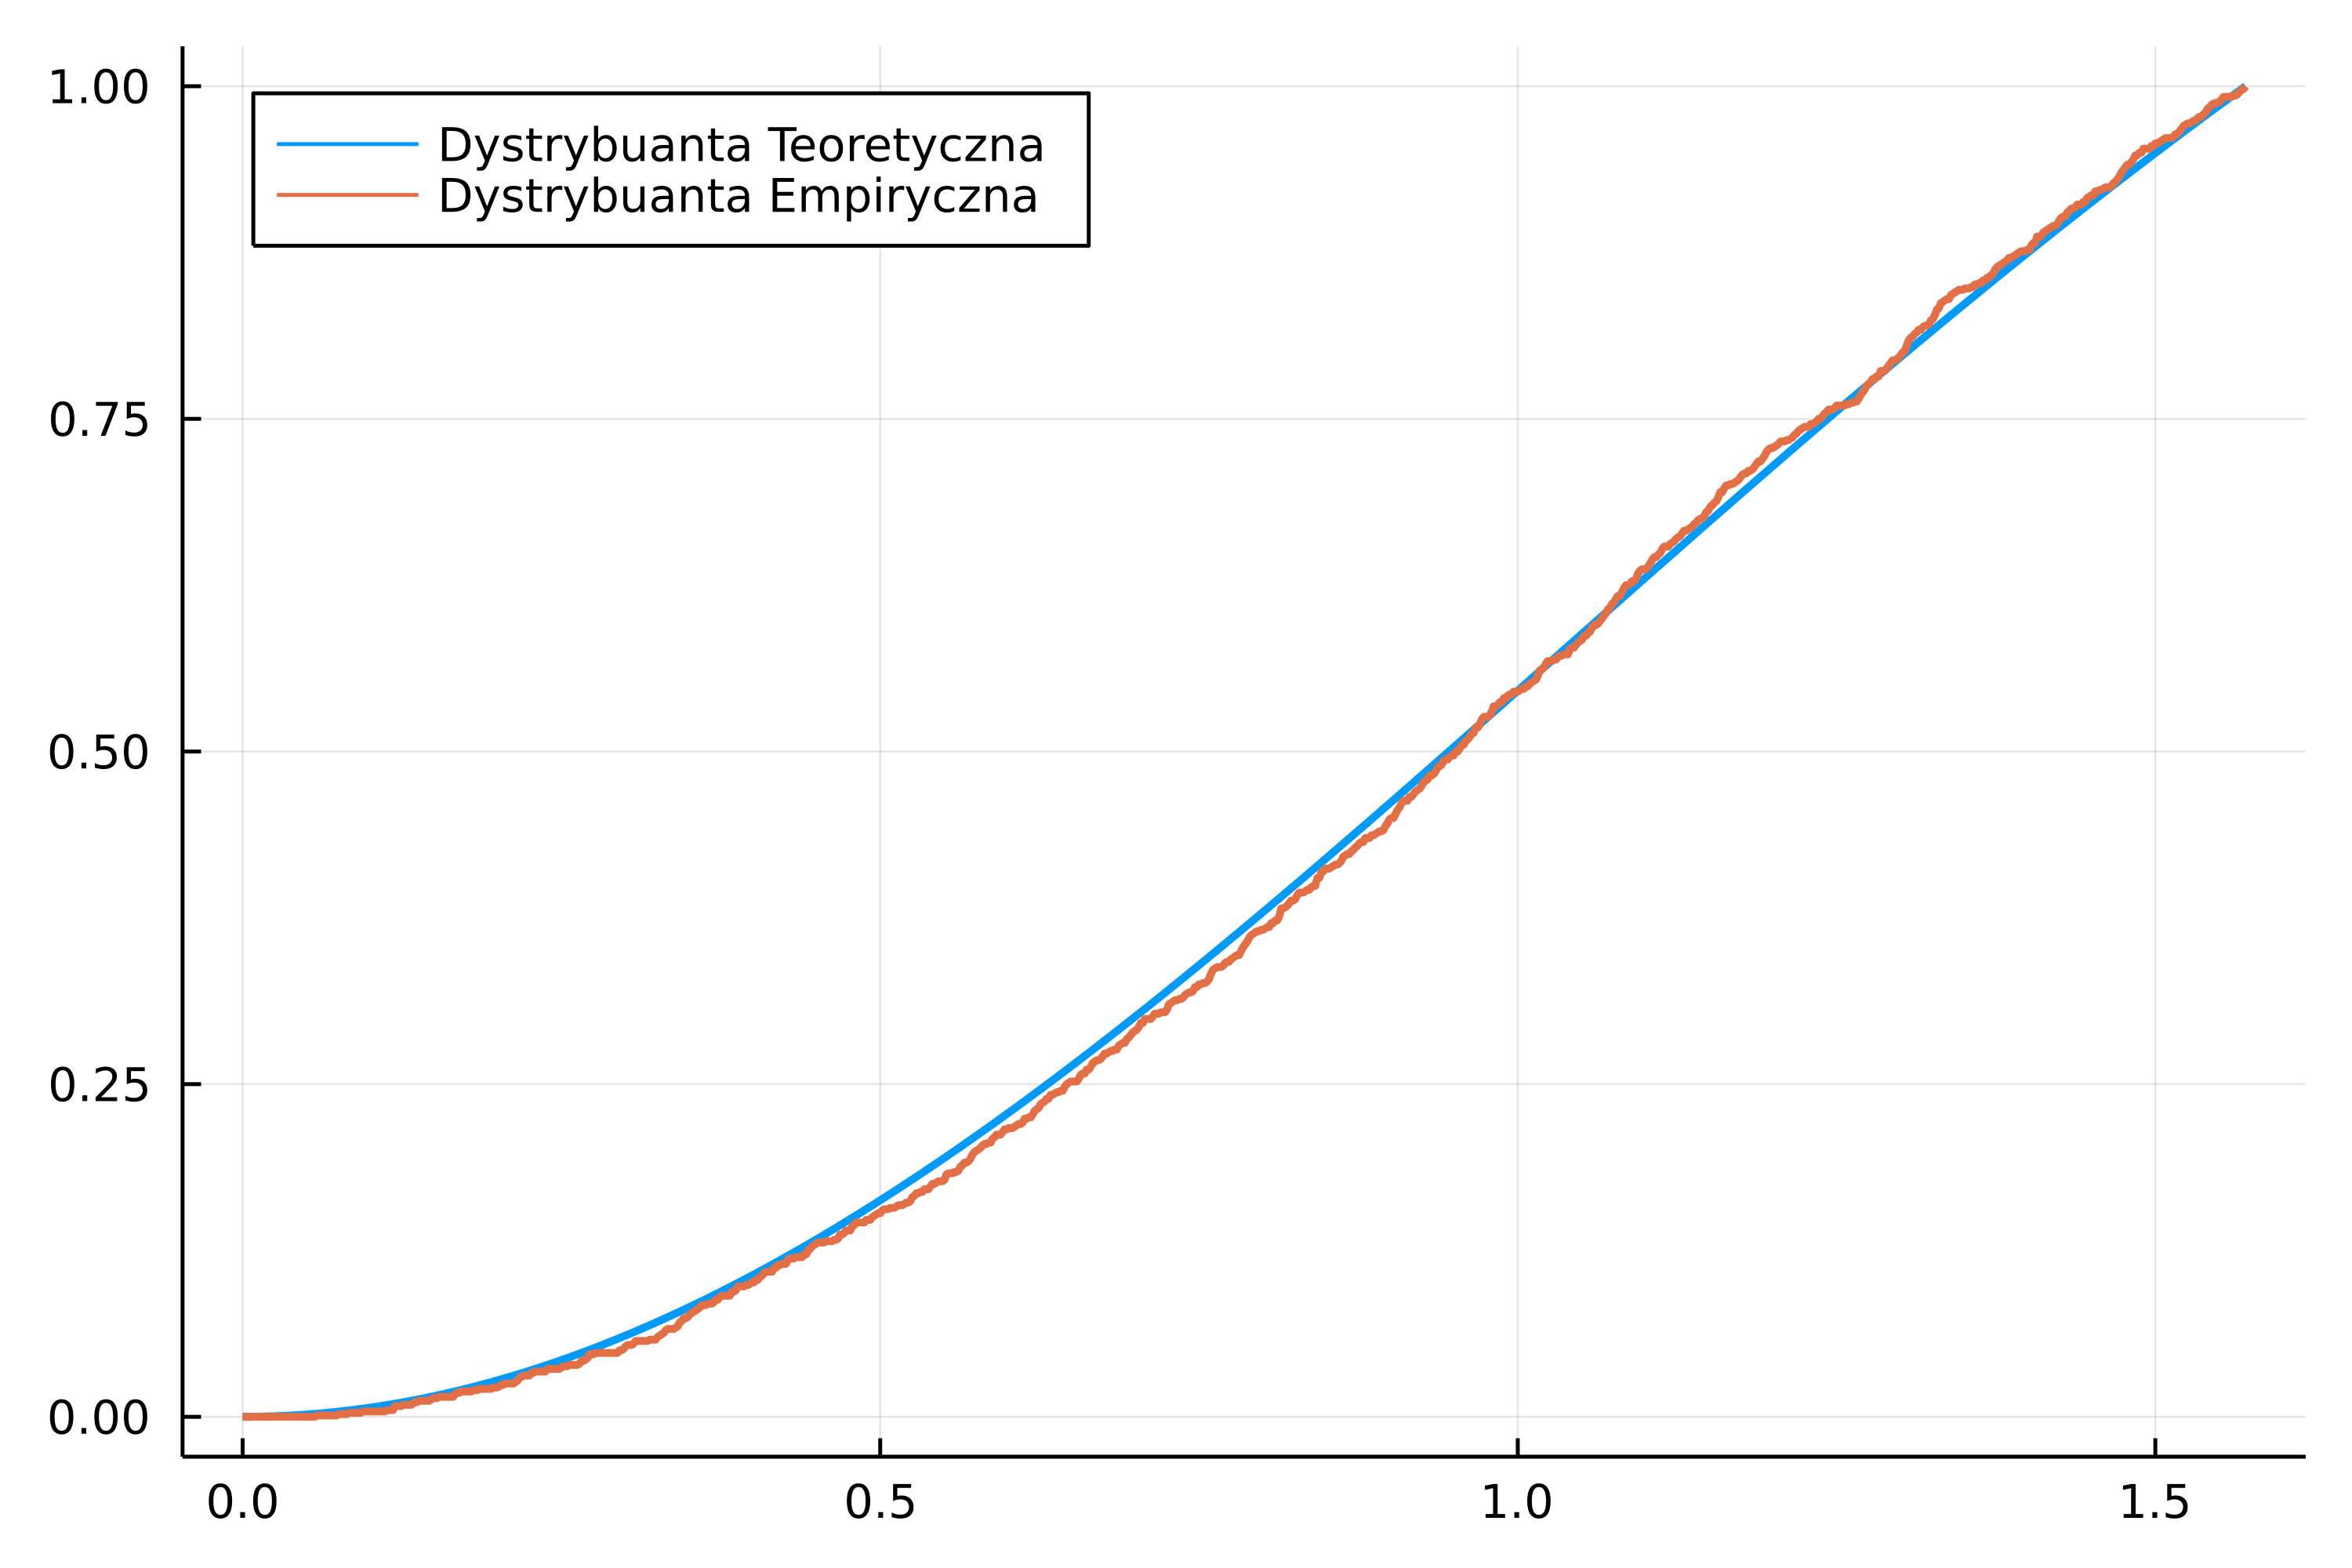
\includegraphics[width=\columnwidth/2-10mm]{fig/fig_AO_con_cdf.png} }}%
%		\qquad
%		\subfloat[\centering label 2]{{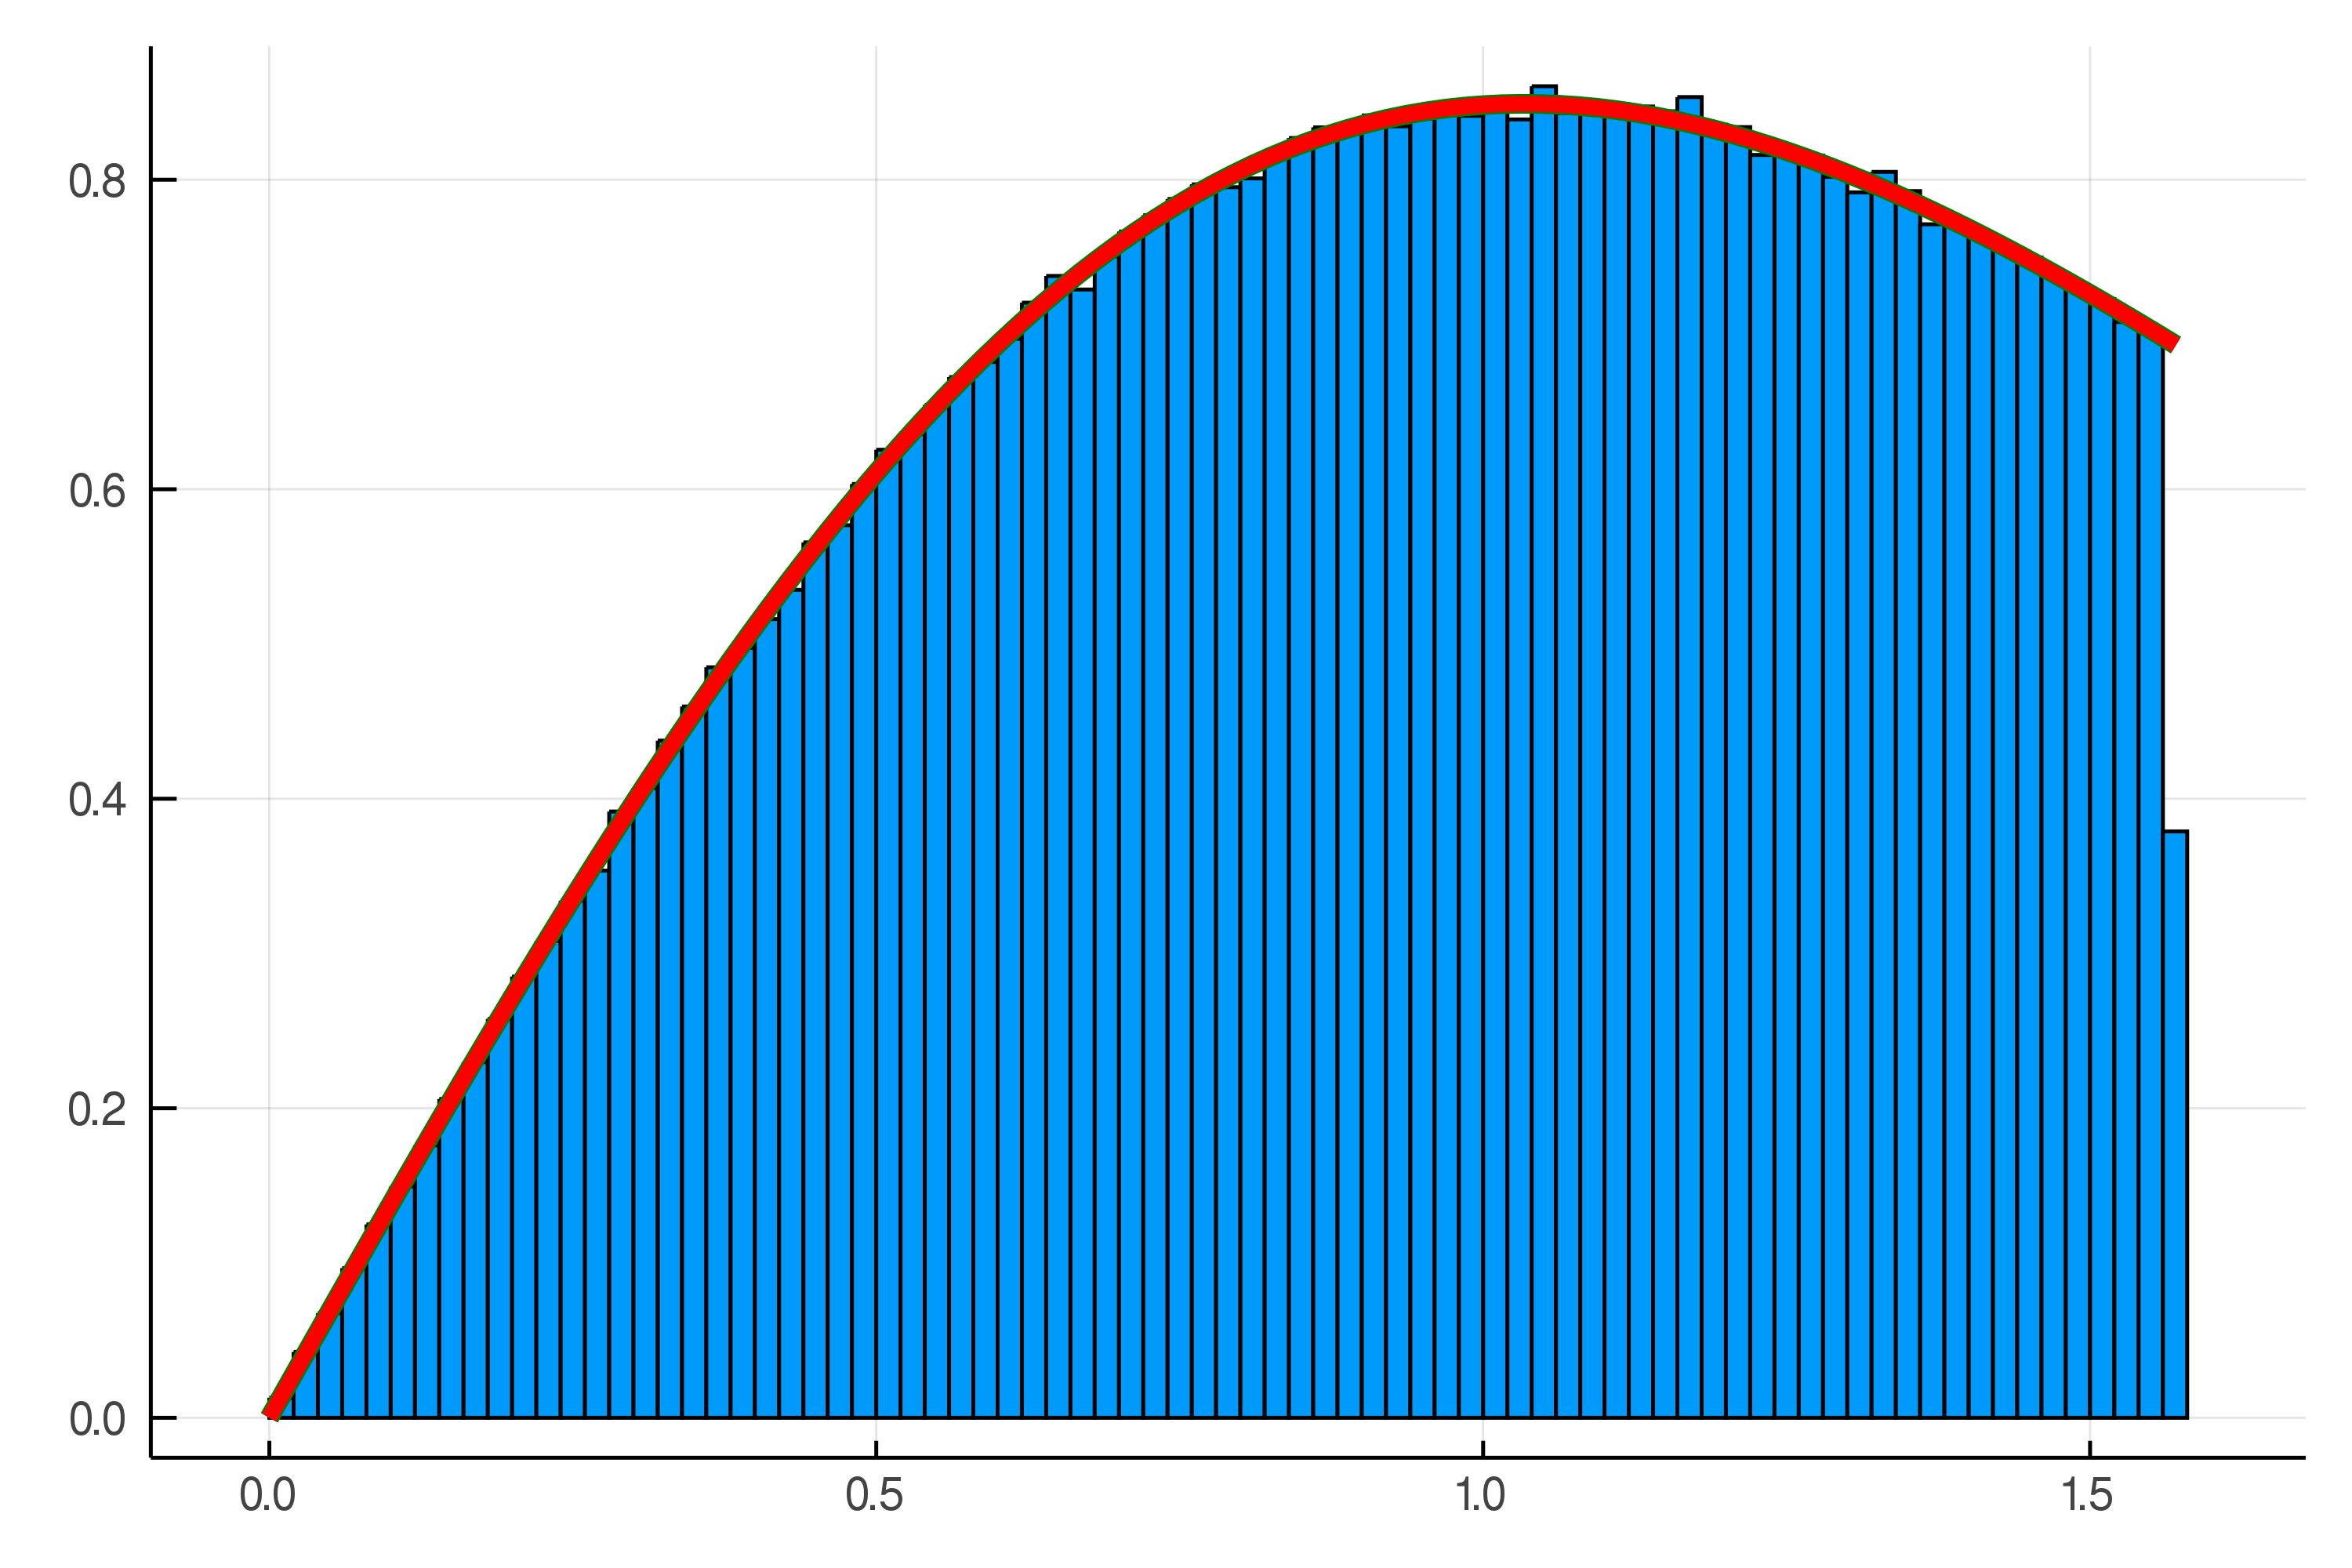
\includegraphics[width=\columnwidth/2-10mm]{fig/fig_AO_con_hist.png} }}%
%		\caption{2 Figures side by side}%
%		\label{fig:example}%
%	\end{figure}









%%%%%%%%%%%%%%%%%%%%%%%%%%%%%%%%%%%%%%%%3
	
	\section{Metoda splotowa\textsuperscript{\cite{splot}}}
	
	\subsection{Opis}
	\noindent Metoda ta pozwala wygenerować pewną zmienną losową $X$, przy pomocy innych zmiennych, które potrafimy efektywnie generować, i zsumowaniu ich. Załóżmy, że
	$$ X \buildrel{d} \over{=} Y_1 + Y_2 + \dots + Y_n, $$
	gdzie $Y_i$ to zmienne losowe niezależne. Wtedy algorytm wygląda następująco:
	\begin{enumerate}[leftmargin=10mm]
		\item Generuj $ Y_1, Y_2, \dots, Y_n $.
		\item Zwróć $ X = Y_1 + Y_2 + \dots + Y_n $.
	\end{enumerate}

	\subsection{Przykłady}
	
	\subsubsection{Dyskretny - rozkład dwumianowy}
	\noindent Niech $ X \sim \mathcal{B}(n, p) $ oraz niech $Y_1, Y_2, \dots, Y_n$ będzie ciągiem niezależnych zmiennych losowych będących wynikami prób Bernoulliego z prawdopodobieństwem sukcesu $p$. Wtedy
	$$ X \buildrel{d} \over{=} Y_1 + Y_2 + \dots + Y_n. $$
	Stąd mamy algorytm:
	\begin{enumerate}[leftmargin=10mm]
		\item Generuj $ Y_1, Y_2, \dots, Y_n $, gdzie $Y_i \sim \mathcal{B}(1, p) $.
		\item Zwróć $ X = Y_1 + Y_2 + \dots + Y_n $.
	\end{enumerate}
	\begin{figure}[H]
		\centering
		\caption{Porównanie dystrybuanty empirycznej i teoretycznej dla próby z rozkładu $\mathcal{B}(500, \frac{3}{10})$ o długości $n = 1000$.}
		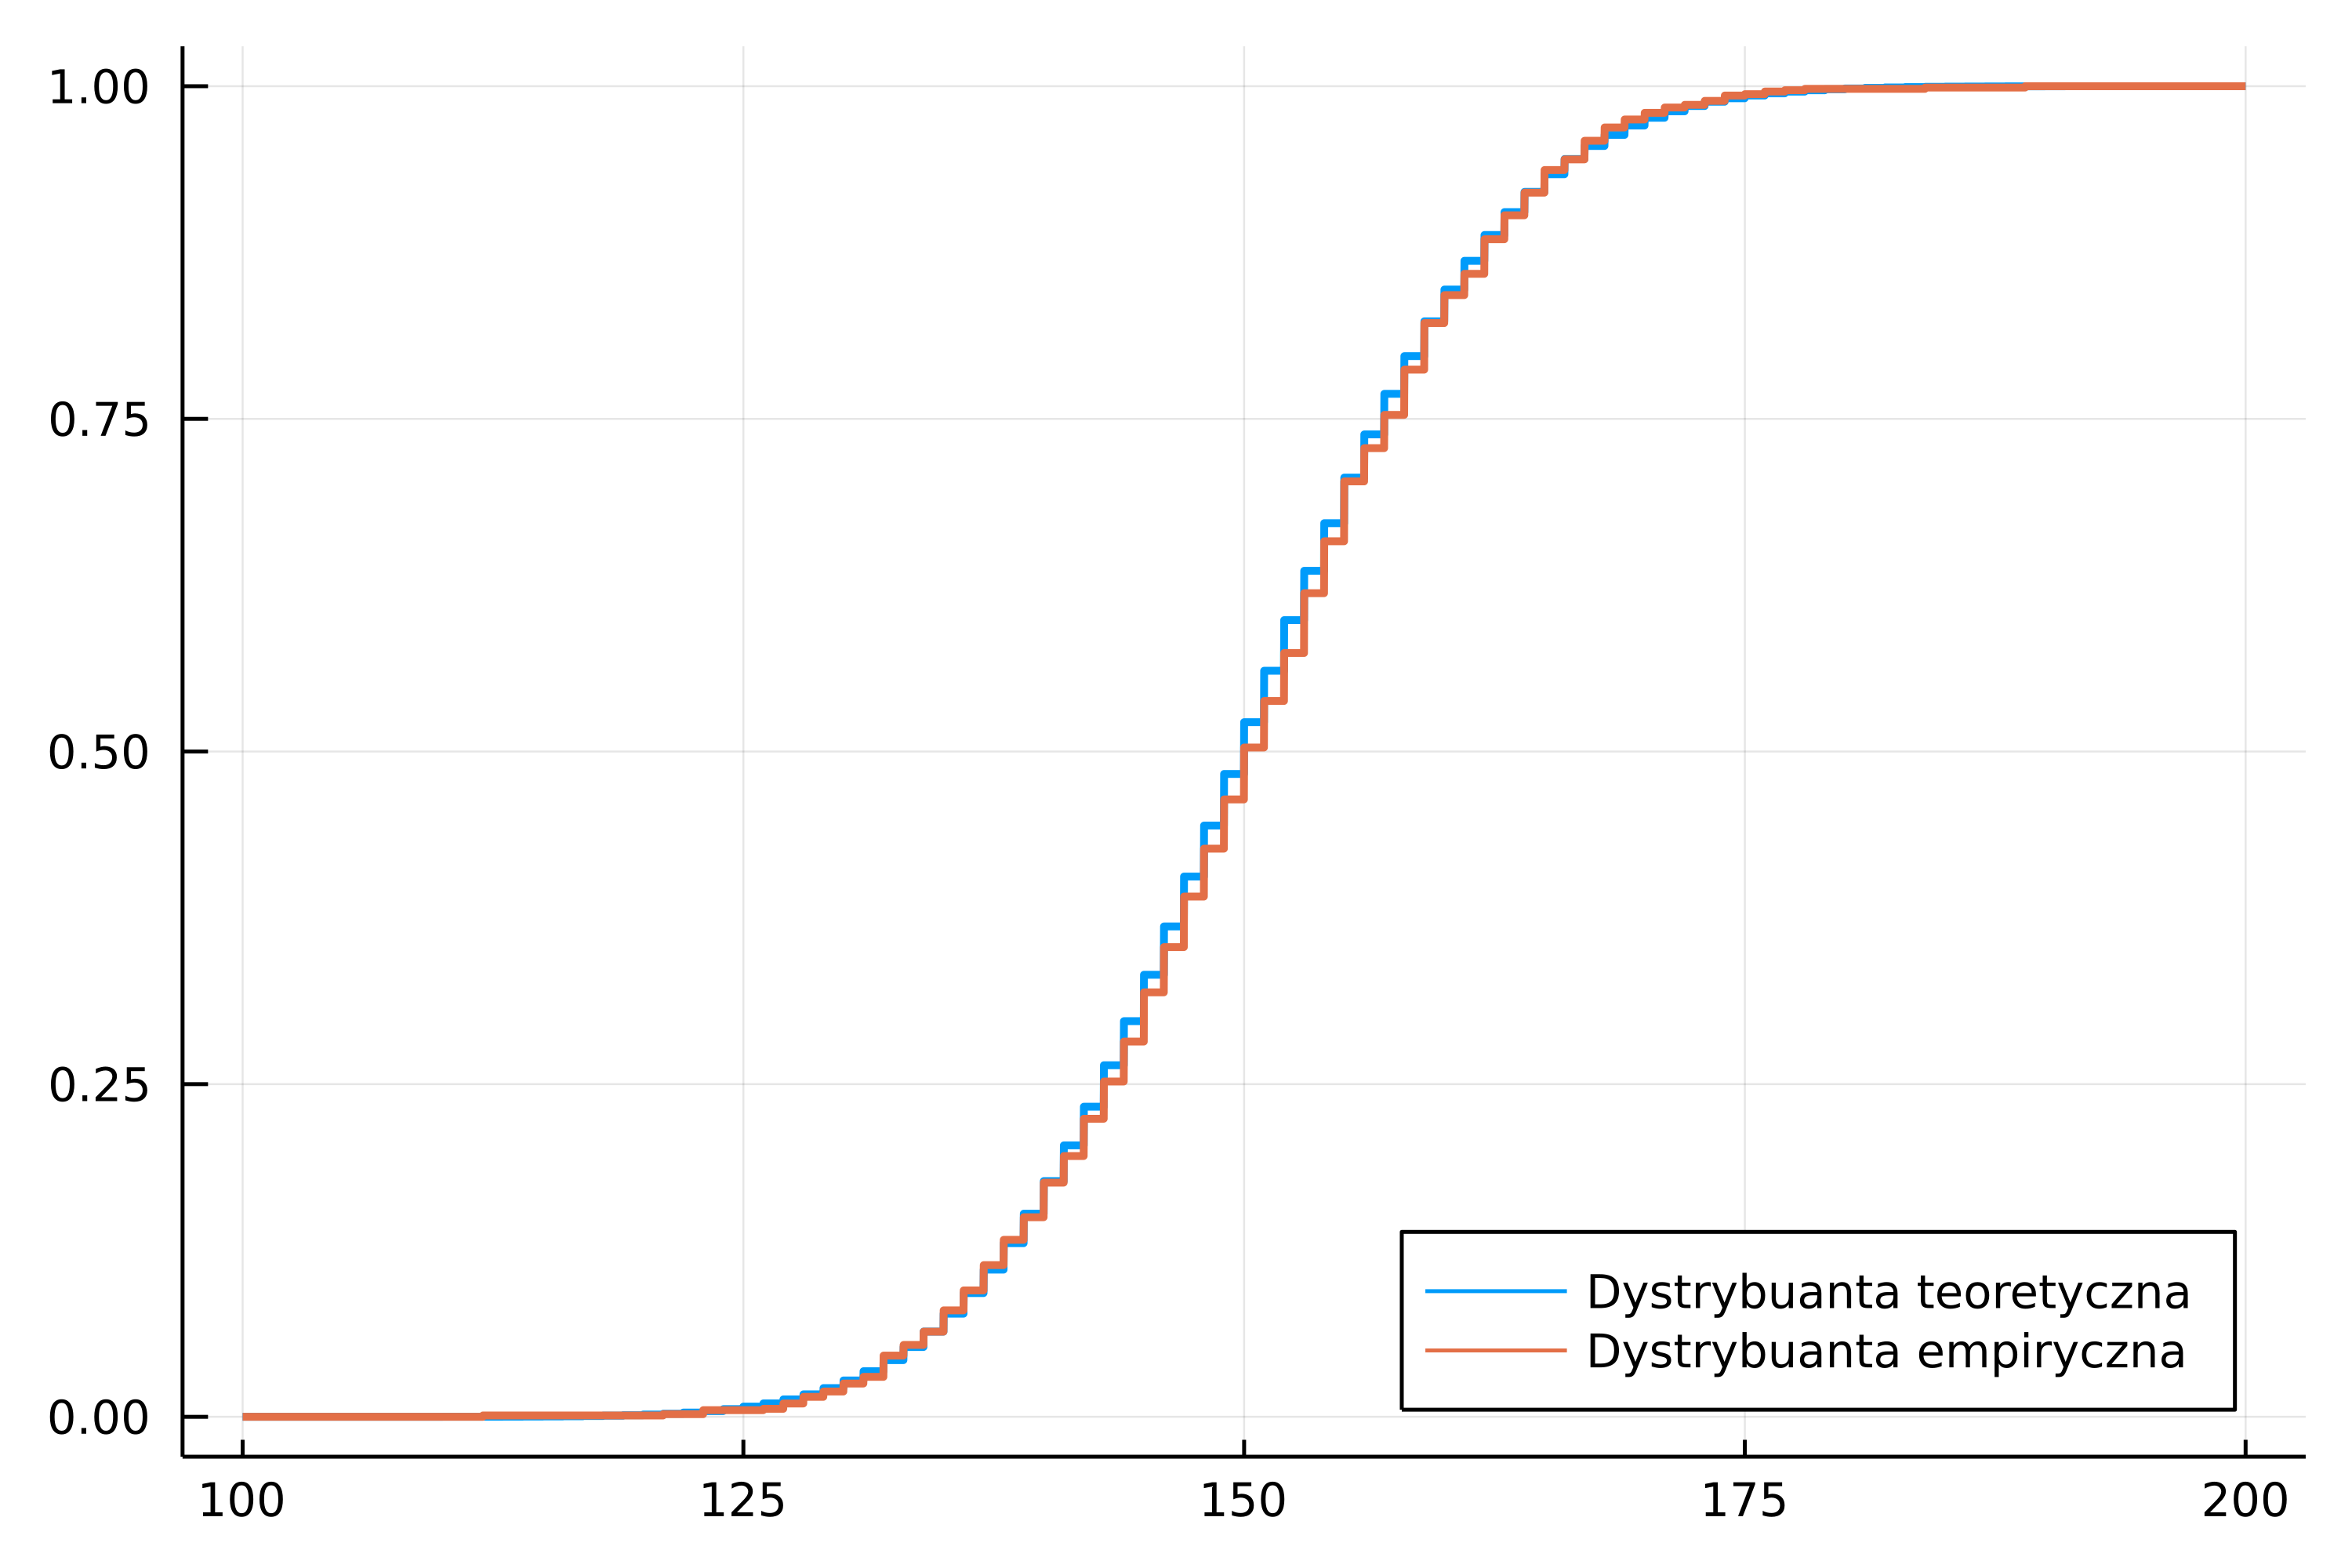
\includegraphics[scale=0.1]{fig/fig_splot1.png}
	\end{figure}
	
	\subsubsection{Ciągły - rozkład chi-kwadrat}
	\noindent Niech $ X \sim \mathcal{X}^2(n) $ oraz niech $Y_1, Y_2, \dots, Y_n$ będzie ciągiem niezależnych zmiennych losowych o rozkładzie normalnym standardowym. Wtedy
	$$ X \buildrel{d} \over{=} Y_1^2 + Y_2^2 + \dots + Y_n^2. $$
	Stąd otrzymujemy algorytm:
	\begin{enumerate}[leftmargin=10mm]
		\item Generuj $ Y_1, Y_2, \dots, Y_n $, gdzie $Y_i \sim \mathcal{N}(0, 1) $.
		\item Zwróć $ X = Y_1^2 + Y_2^2 + \dots + Y_n^2 $.
	\end{enumerate}
	\begin{figure}[H]
		\centering
		\caption{Porównanie dystrybuanty empirycznej i teoretycznej oraz wykres kwantylowy dla próby z rozkładu $\mathcal{X}^2(10)$ o długości $n = 1000$.}
		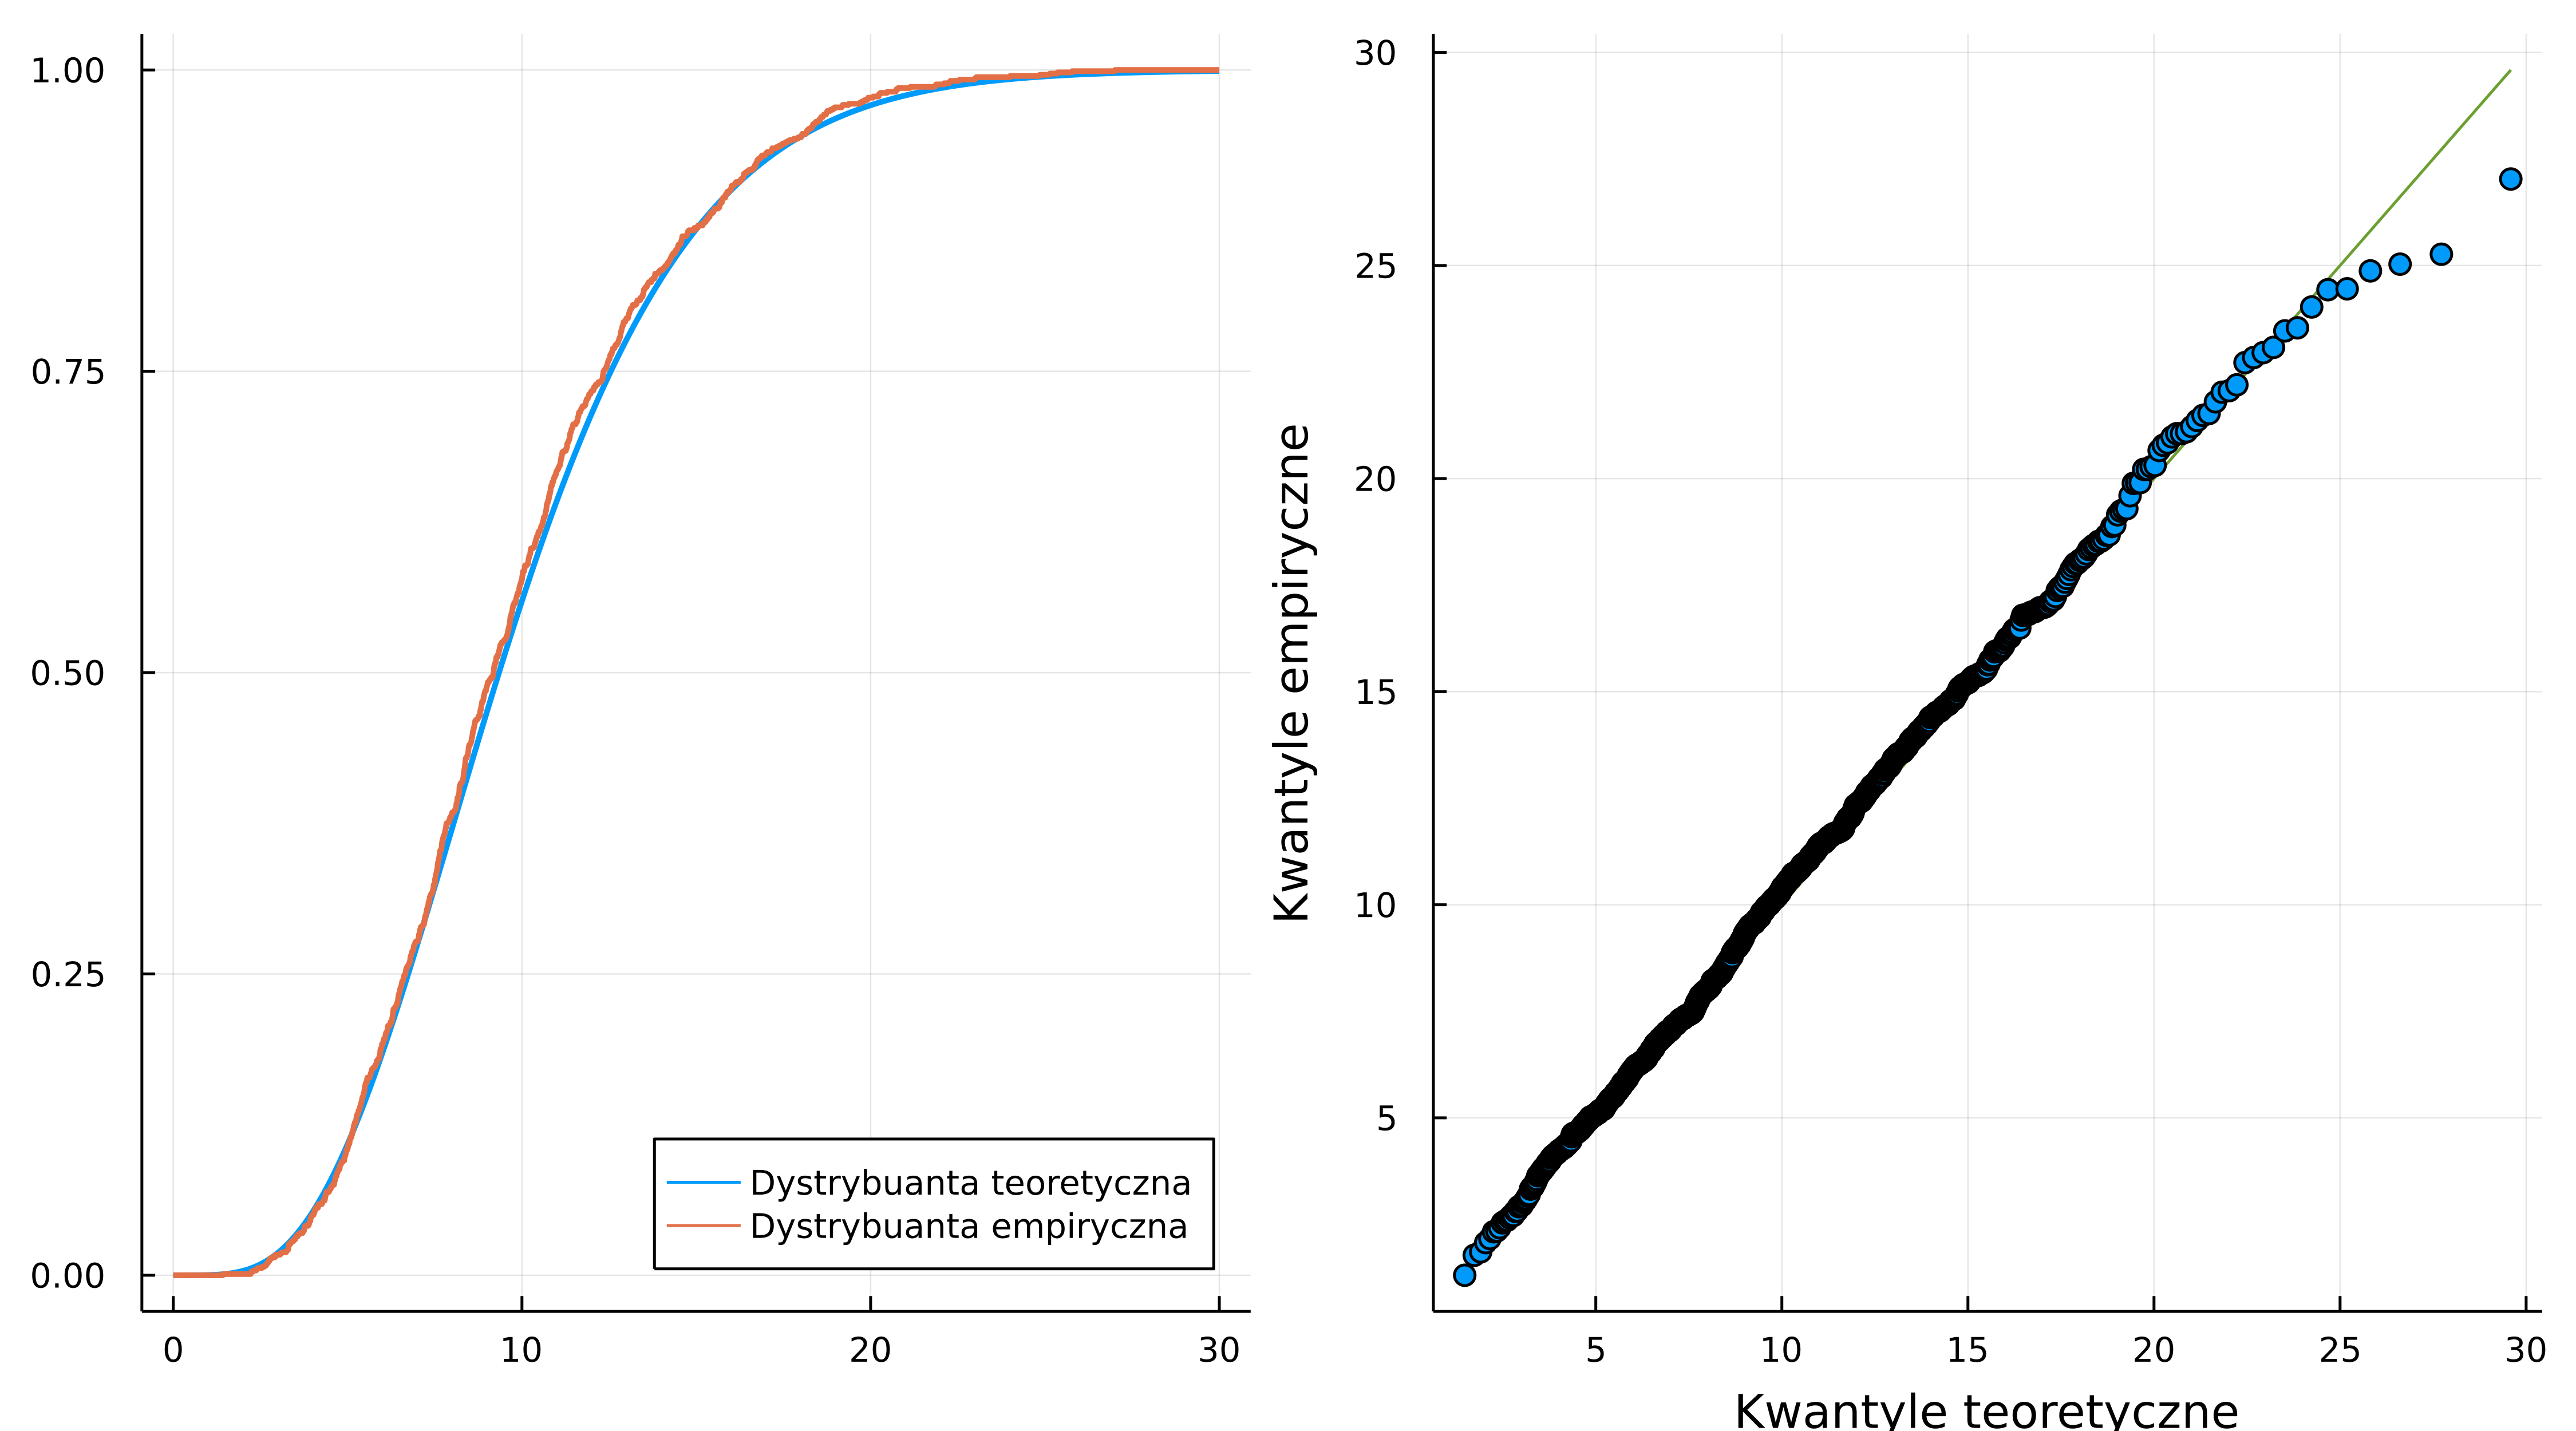
\includegraphics[scale=0.1]{fig/fig_splot2.png}
	\end{figure}
	
	
	
	
	
	\section{Metoda kompozycji\textsuperscript{\cite{kompozycja}}}
	
	\subsection{Opis}
	\noindent Metoda ta służy do generowania wyłącznie ciągłych rozkładów. Załóżmy, że zmienna losowa $X$, którą chcemy symulować, ma dystrybuantę postaci
	$$ F(x) = \sum_{i=1}^n p_i F_i(x), $$
	gdzie $p_i > 0$, \ $\sum\limits_{i=1}^n p_i = 1$ oraz $F_i$ to dystrybuanty pewnych zmiennych losowych $Y_i$. Jeżeli zmienne $Y_i$ mają gęstość, to równoważne będzie założenie, że gęstość zmiennej $X$ ma postać
	$$ f(x) = \sum_{i=1}^n p_i f_i(x), $$
	gdzie $f$ są gęstościami zmiennych $Y_i$. Do wygenerowania $X$ może posłużyć poniższy algorytm:
	\begin{enumerate}[leftmargin=10mm]
		\item Generuj zmienną losową $I$ o rozkładzie $\mathrm{P}(I = i) = p_i$.
		\item Generuj $Y_I$.
		\item Zwróć $X = Y_I$.
	\end{enumerate}

	\subsection{Przykład}
	\noindent Chcemy wygenerować zmienną losową $X$ o gęstości
	$$ f(x) = \frac{1}{3\pi(1 + x^2)} + \frac{2}{3\sqrt{2\pi}}\mathrm{e}^{-\frac{x^2}{2}}. $$
	Jeśli zapiszemy ją w postaci
	$$ f(x) = \frac{1}{3}\left(\frac{1}{\pi(1 + x^2)} \right) + \frac{2}{3}\left(\frac{1}{\sqrt{2\pi}}\mathrm{e}^{-\frac{x^2}{2}}\right), $$
	to możemy zauważyć, że jest to suma gęstości rozkładów Cauchy'ego i normalnego standardowego. Weźmy zatem $Y_1 \sim \mathcal{C}(0, 1)$ oraz $Y_2 \sim \mathcal{N}(0, 1)$. Niech $p_1 = \frac{1}{3}$ i $p_2 = \frac{2}{3}$. Wtedy możemy zapisać
	$$ f(x) = p_1 f_1(x) + p_2 f_2(x), $$
	gdzie $f_1$ i $f_2$ to gęstości odpowiednio $Y_1$ i $Y_2$. Stąd algorytm prezentuje się następująco:
	\begin{enumerate}[leftmargin=10mm]
		\item Generuj $I$ o rozkładzie $\mathrm{P}(I = 1) = \frac{1}{3}$, \ $\mathrm{P}(I = 2) = \frac{2}{3}$.
		\item Generuj $Y_I$.
		\item Zwróć $X = Y_I$.
	\end{enumerate}
	\begin{figure}[H]
		\centering
		\caption{Porównanie histogramu z gęstością teoretyczną oraz porównanie dystrybuanty empirycznej i teoretycznej dla próby z powyższego rozkładu mieszanego o długości $n = 1000$.}
		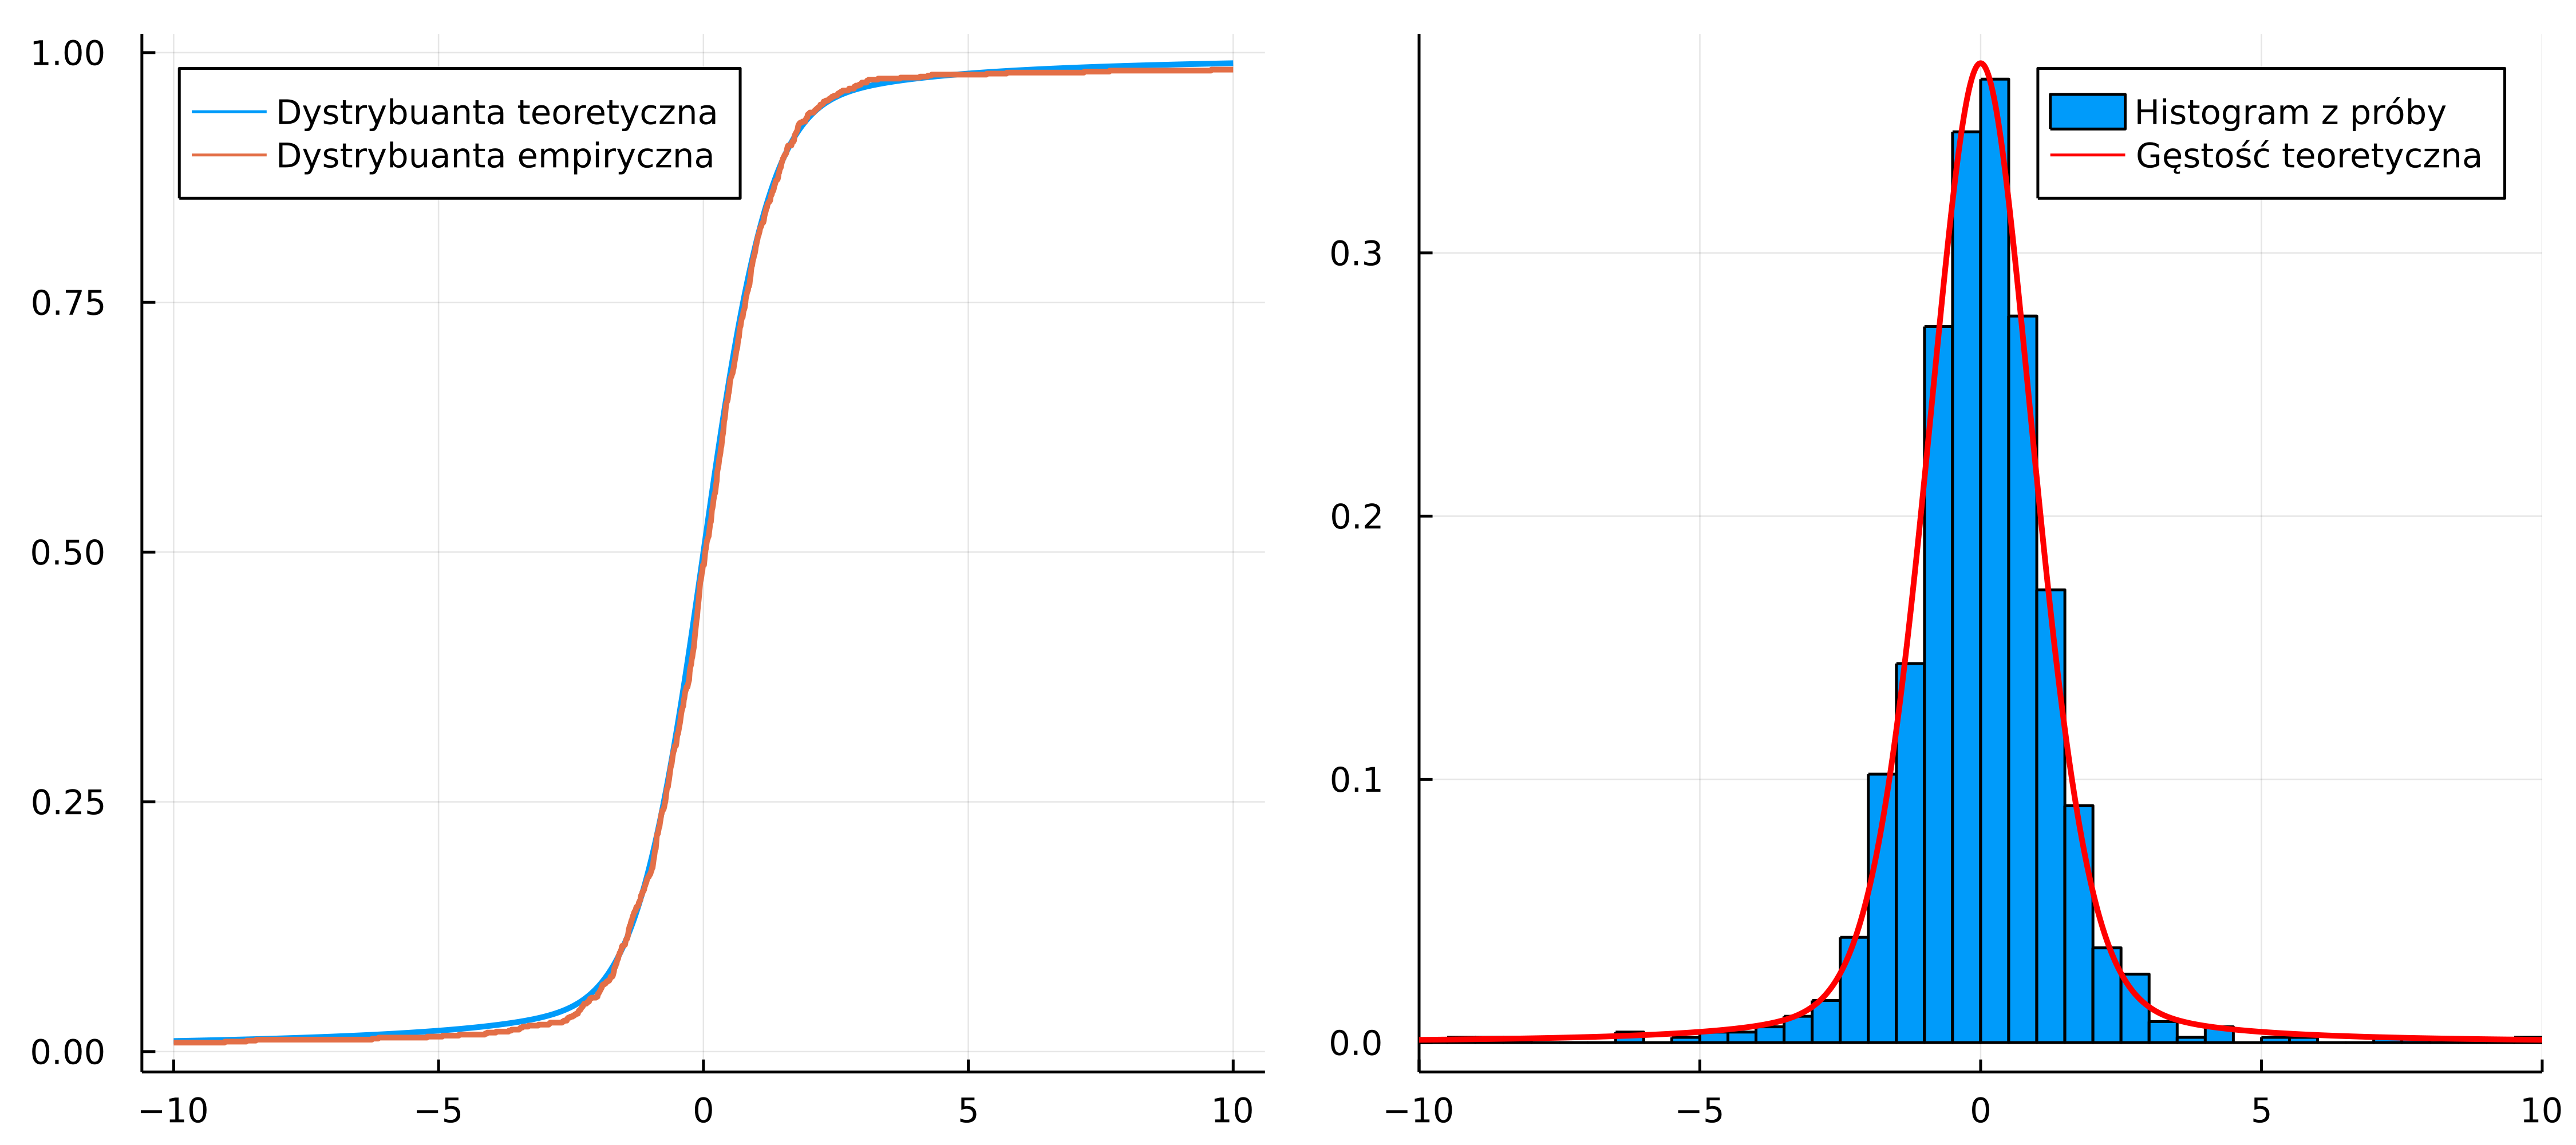
\includegraphics[scale=0.1]{fig/fig_komp.png}
	\end{figure}



%%%%%%%%%%%%%%%%%%%%%%%%%%%%%%%%%%%%%%%%4
	
	\section{Metoda Boxa-M{u}llera\textsuperscript{\cite{box-kox}} - Budnik}
	\subsection{Opis}
	\noindent Najważniejszym rozkładem w prawdopodobieństwie jest rozkład normalny. Dlatego istnieje specjalna metoda generowania jego. Łatwo można pokazać (co zrobiliśmy na kursie Modelowanie Stochastyczne), że jeśli $U_1,U_2$ - iid, $U_1\sim\mathcal{U}(0,1)$, to zmienne
	\begin{equation}\label{eq:B-M}
		\begin{split}
			X=\sqrt{-2\ln(U_1)}\cos(2\pi U_2)\\
			Y=\sqrt{-2\ln(U_1)}\sin(2\pi U_2)
		\end{split}
	\end{equation}
	są niezależne oraz obie mają rozkład normalny standardowy $\mathcal{N}(0,1)$. Na tej podstawie powstał poniższy algorytm
	\subsubsection{Algorytm}
	\begin{enumerate}[leftmargin=10mm]
		\item Generuj zmienne $U_1, U_2$ - iid, $U_1\sim\mathcal{U}(0,1)$
		\item Zwróć:
		\begin{equation}
			\begin{split}
				X=\sqrt{-2\ln(U_1)}\cos\left(2\pi U_2\right)\\
				Y=\sqrt{-2\ln(U_1)}\sin\left(2\pi U_2\right)
			\end{split}
		\end{equation}
	\end{enumerate}
	Algorytm ten generuje od razu dwie próby z rozkładu normalnego standardowego. By wygenerować zmienną z rozkładu $\mathcal{N}(\mu,\sigma^2)$ wystarczy wcześniej wygenerowane zmienne pomnożyć przez $\sigma$ po czym dodać do nich $\mu$.
	\subsection{Przykłady}
	
	\begin{figure}[H]\caption{Sprawdzenie poprawności metody Boxa-Mullera dla próby o rozmiarze $n=1000$}\label{fig:BM}
		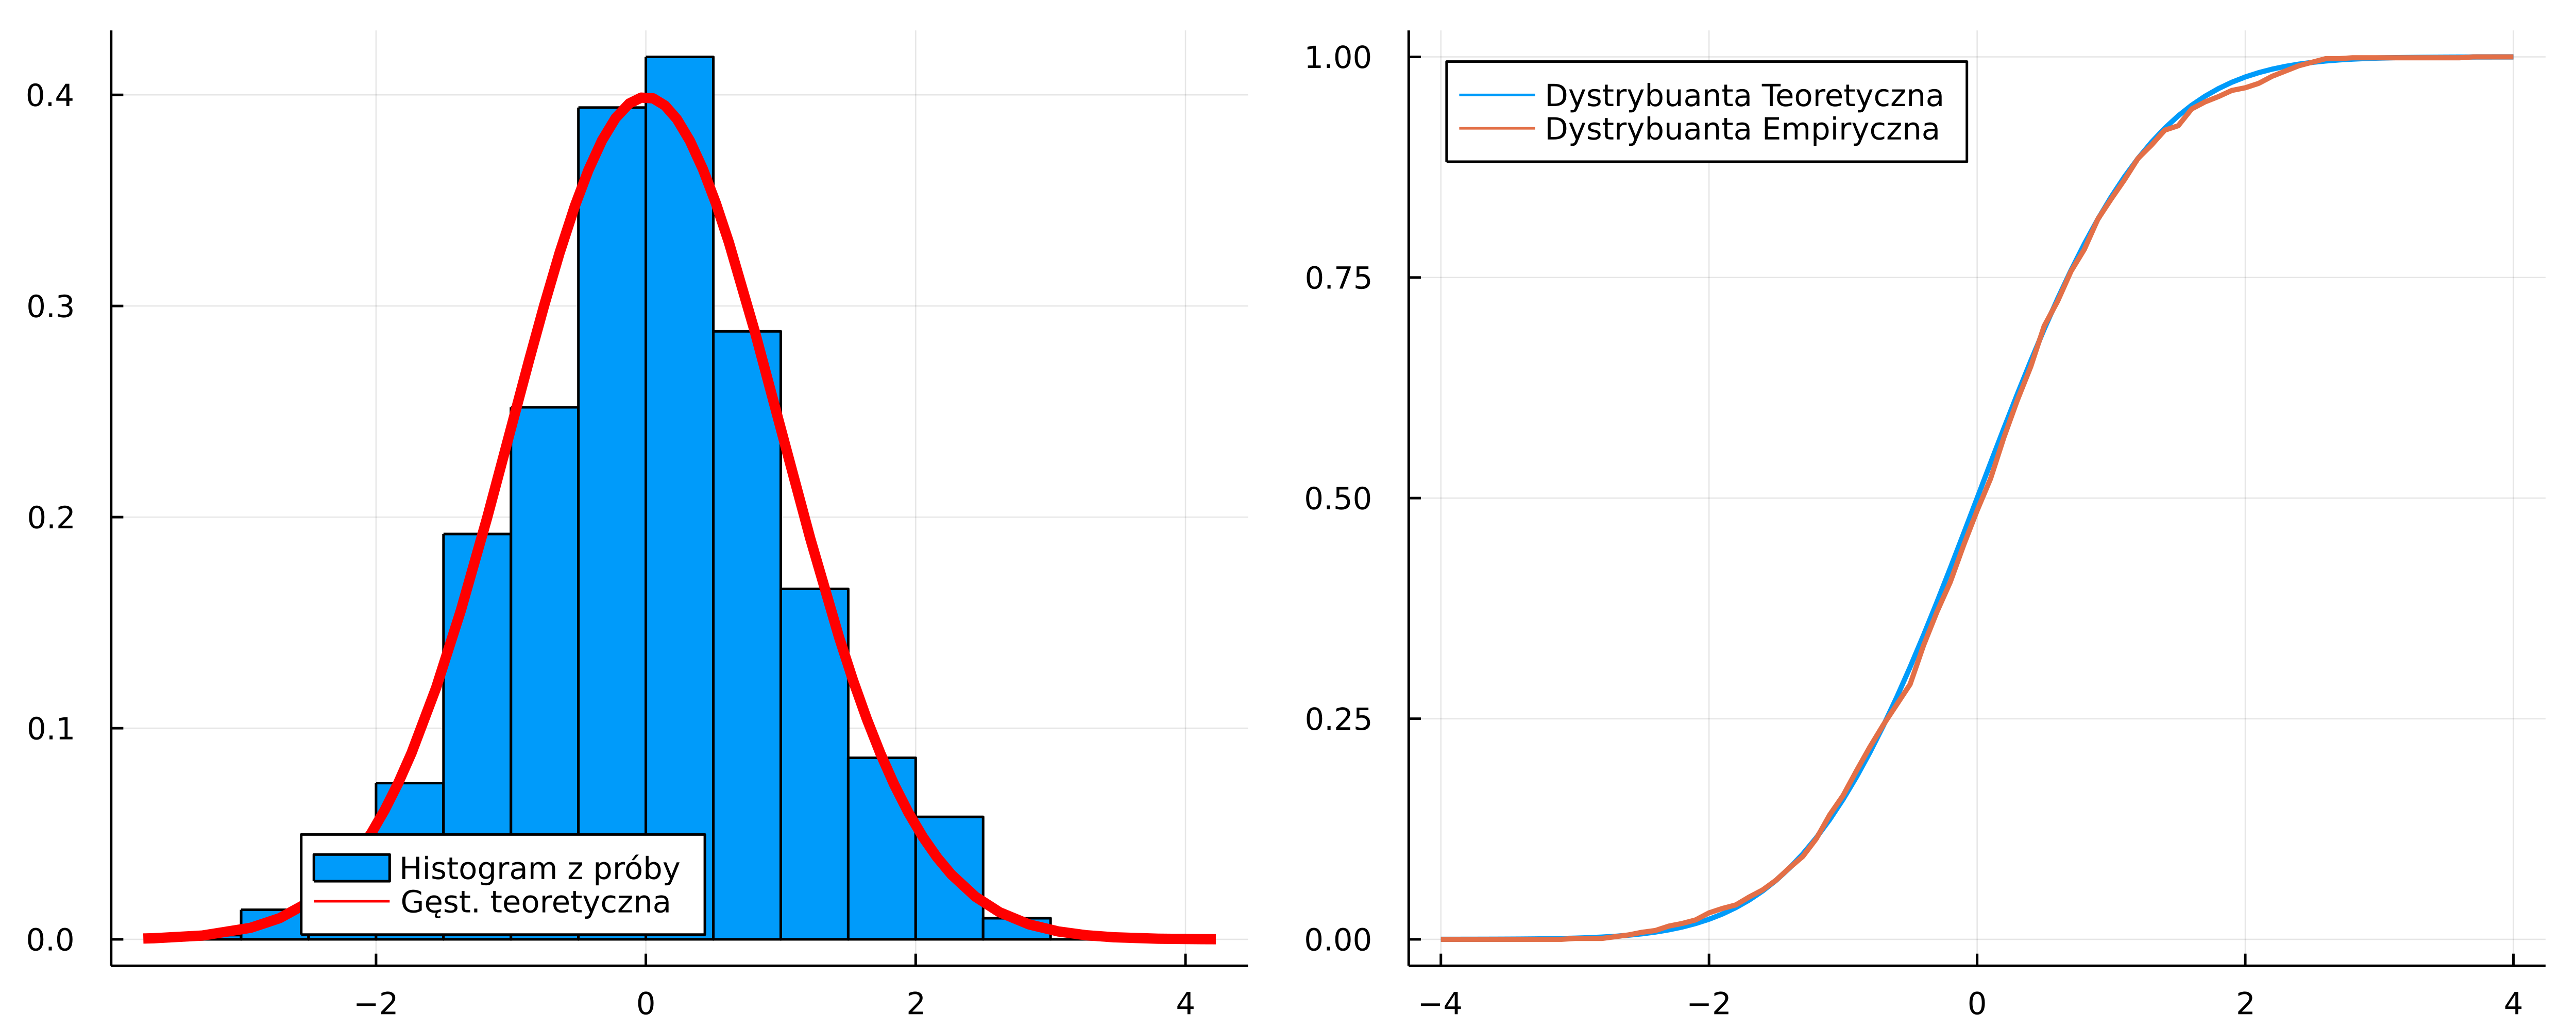
\includegraphics[width=\columnwidth]{fig/fig_BM.png}
	\end{figure}
	
	
	
	\section{Metoda biegunowa\textsuperscript{\cite{polar}} - Budink}
	\subsection{Opis}
	\noindent Jak wspomnieliśmy poprzednio rozkład normalny jest najważniejszym rozkładem prawdopodobieństwa. Z tego powodu jest on bardzo często wykorzystywany, ważne jest by generowanie próby trwało jak najkrócej. Niestety w metodzie Boxa-M{u}llera wyznaczanie pojawiają się funkcje $\sin$ oraz $\cos$. Wyznaczenie ich wartości jest stosunkowo czasochłonne dla procesora, dlatego była poszukiwana metoda, w która nie zawiera tych funkcji. Przekształcając wzór wykorzystywany w metodzie Boxa-Mullera można pokazać, że jeśli wektor $(V_1, V_2)$ ma rozkład jednostajny na kole jednostkowym to zmienne
	\begin{equation}
		\begin{split}
			X=\sqrt{\frac{-2\ln R^2}{R^2}}V_1\\
			Y=\sqrt{\frac{-2\ln R^2}{R^2}}V_2
		\end{split}
	\end{equation}
	mają rozkład normalny standardowy $\mathcal{N}(0,1)$ oraz $X \indep Y$. Ponieważ umiemy w sposób efektywny generować wektor losowy $(V_1, V_2)$ wystarczy skorzystać z poniższego algorytmu
	\subsubsection{Algorytm}
	\begin{enumerate}[leftmargin=10mm]
		\item Generuj zmienne $V_1, V_2$ - iid, $V_1\sim\mathcal{U}(-1,1)$
		\item Wyznacz $R^2=V_1^2+V_2^2$
		\item Jeżeli $R^2\ge 1$ wróć do 1.
		\item Zwróć
		\begin{equation}
			\begin{split}
				X=\sqrt{\frac{-2\ln R^2}{R^2}}V_1\\
				Y=\sqrt{\frac{-2\ln R^2}{R^2}}V_2
			\end{split}
		\end{equation}
	\end{enumerate}
	Podobnie jak w metodzie Boxa-M{u}llera algorytm ten zwraca dwie zmienne niezależne z rozkładu normalnego, więc by otrzymać zmienne z rozkładu $\mathcal{N}(\mu,\sigma^2)$ tak samo jak wcześniej mnożymy wygenerowaną próbę przez $\sigma$ i dodajemy do niej $\mu$.
	
	\subsection{Szybkość algorytmu}
	\noindent Do wygenerowania dwóch prób rozkładu normalnego korzystając z tego algorytmu potrzebne jest powtórzenie go średnio $\frac{4}{\pi}\approx1.25$ razy. Pomimo, że algorytm będzie czasem wykonywany wielokrotnie, to poprzez pozbycie się funkcji trygonometrycznych czas rzeczywisty wygenerowania danej próby będzie krótszy niż w poprzedniej metodzie, co pokażemy później.
	
	\subsection{Przykłady}

	\begin{figure}[H]\caption{Sprawdzenie poprawności metody biegunowej dla próby o rozmiarze $n=1000$}\label{fig:pol}
		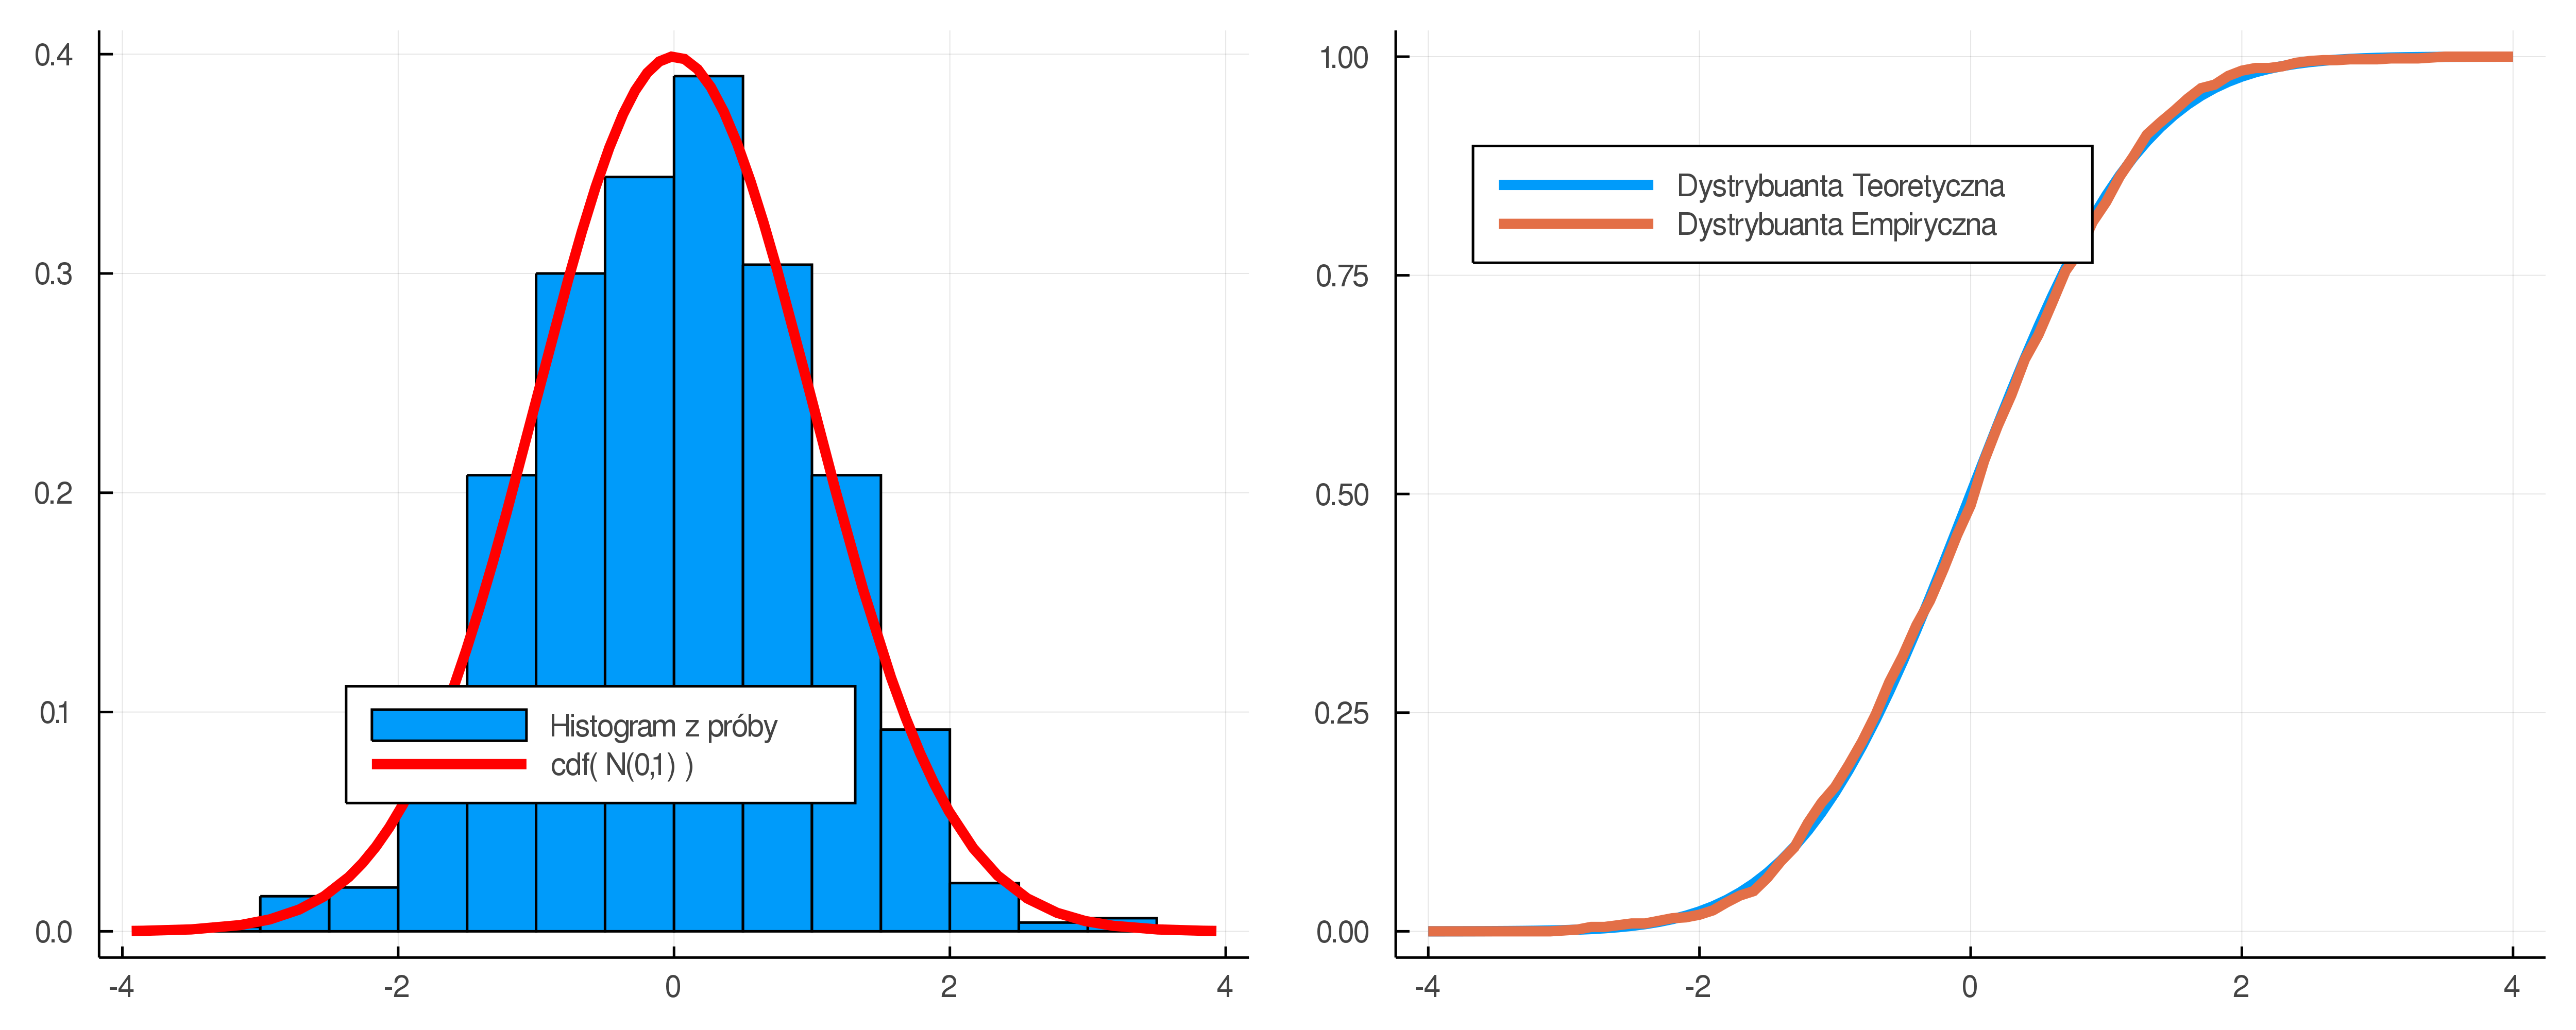
\includegraphics[width=\columnwidth]{fig/fig_pol.png}
	\end{figure}

	\section{Porównanie metod generowania rozkładu normalnego}
	\noindent Dwie ostatnie metody jakie pokazaliśmy dotyczą generowania tego samego rozkładu, dlatego ważne wydaje się, by porównać czas ich działania. Wykonaliśmy pomiary czasu generowania różnych wielkości prób (o wielkości $N$) dla metody Boxa-Mullera (B-M) oraz metody biegunowej. Dodatkowo policzyliśmy stosunek czasu potrzebnego do wygenerowania próby metodą B-M do czasu przy użyciu metody biegunowej. Dla wartości do $2^{24}$ pomiar wykonaliśmy 1000 razy, dla liczb nie większych niż $2^{27}$ zmniejszyliśmy pomiar do 200 prób, a pozostałe wielkości prób wygenerowaliśmy jedynie 10 razy. Wyniki pomiarów 
	\begin{table}[H]\caption{Czas wykonania danych metod dla danych wielkości prób}\label{tab:time}
		\begin{tabularx}{\textwidth}{|Z{6mm}|Z{19mm}|Y|Y|p{5mm}|Z{6mm}|Z{19mm}|Y|Y|}
			\cline{1-4}\cline{6-9}
			$N$      & Biegunowa & B-M&Stosunek& $\vphantom{\dfrac{1}{1}}$ & $N$      & Biegunowa & B-M & Stosunek \\ \cline{1-4}\cline{6-9}
			$2^{11}$ & 0.000076 & 0.000071 & 1.070  &$\vphantom{\dfrac{1}{1}}$&  $2^{20}$ & 0.019 & 0.030 & 0.633\\\cline{1-4}\cline{6-9}
			$2^{12}$ & 0.000094 & 0.000133 & 0.707  &$\vphantom{\dfrac{1}{1}}$&  $2^{21}$ & 0.037 & 0.060 & 0.614\\\cline{1-4}\cline{6-9}
			$2^{13}$ & 0.000189 & 0.000285 & 0.663  &$\vphantom{\dfrac{1}{1}}$&  $2^{22}$ & 0.076 & 0.115 & 0.663\\\cline{1-4}\cline{6-9}
			$2^{14}$ & 0.000295 & 0.000529 & 0.558  &$\vphantom{\dfrac{1}{1}}$&  $2^{23}$ & 0.149 & 0.231 & 0.647\\\cline{1-4}\cline{6-9}
			$2^{15}$ & 0.000559 & 0.000944 & 0.592  &$\vphantom{\dfrac{1}{1}}$&  $2^{24}$ & 0.326 & 0.440 & 0.742\\\cline{1-4}\cline{6-9}
			$2^{16}$ & 0.000919 & 0.001627 & 0.565  &$\vphantom{\dfrac{1}{1}}$&  $2^{25}$ & 0.659 & 0.974 & 0.677\\\cline{1-4}\cline{6-9}
			$2^{17}$ & 0.001612 & 0.003385 & 0.476  &$\vphantom{\dfrac{1}{1}}$&  $2^{26}$ & 1.316 & 1.821 & 0.723\\\cline{1-4}\cline{6-9}
			$2^{18}$ & 0.004848 & 0.007636 & 0.635  &$\vphantom{\dfrac{1}{1}}$&  $2^{27}$ & 2.836 & 3.990 & 0.711\\\cline{1-4}\cline{6-9}
			$2^{19}$ & 0.009334 & 0.015469 & 0.603  &$\vphantom{\dfrac{1}{1}}$&  $2^{28}$ & 5.500 & 7.786 & 0.706\\\cline{1-4}\cline{6-9}
			$2^{20}$ & 0.018661 & 0.029472 & 0.633  &$\vphantom{\dfrac{1}{1}}$&  $2^{29}$ & 17.157 & 35.594 & 0.482\\\cline{1-4}\cline{6-9}
		\end{tabularx}
	\end{table}
%	\noindent Możemy przedstawić jeszcze te wartości na wykresach. Ponieważ widzimy, że liczba prób rośnie wykładniczo i podejrzewamy, że czas wykonania podobnie możemy nałożyć na obie osie odpowiednie logarytmy. Otrzymujemy w poniższe wykresy
	\noindent Możemy przedstawić jeszcze te wartości na wykresach. Ponieważ wielkości naszej próby rosą wykładniczo na obie osie nałożyliśmy $\log_2$. 
	\begin{figure}[H]\caption{Wykres czasu generowania zmiennych w zależności od wielkości próby}\label{fig:normal_time}
		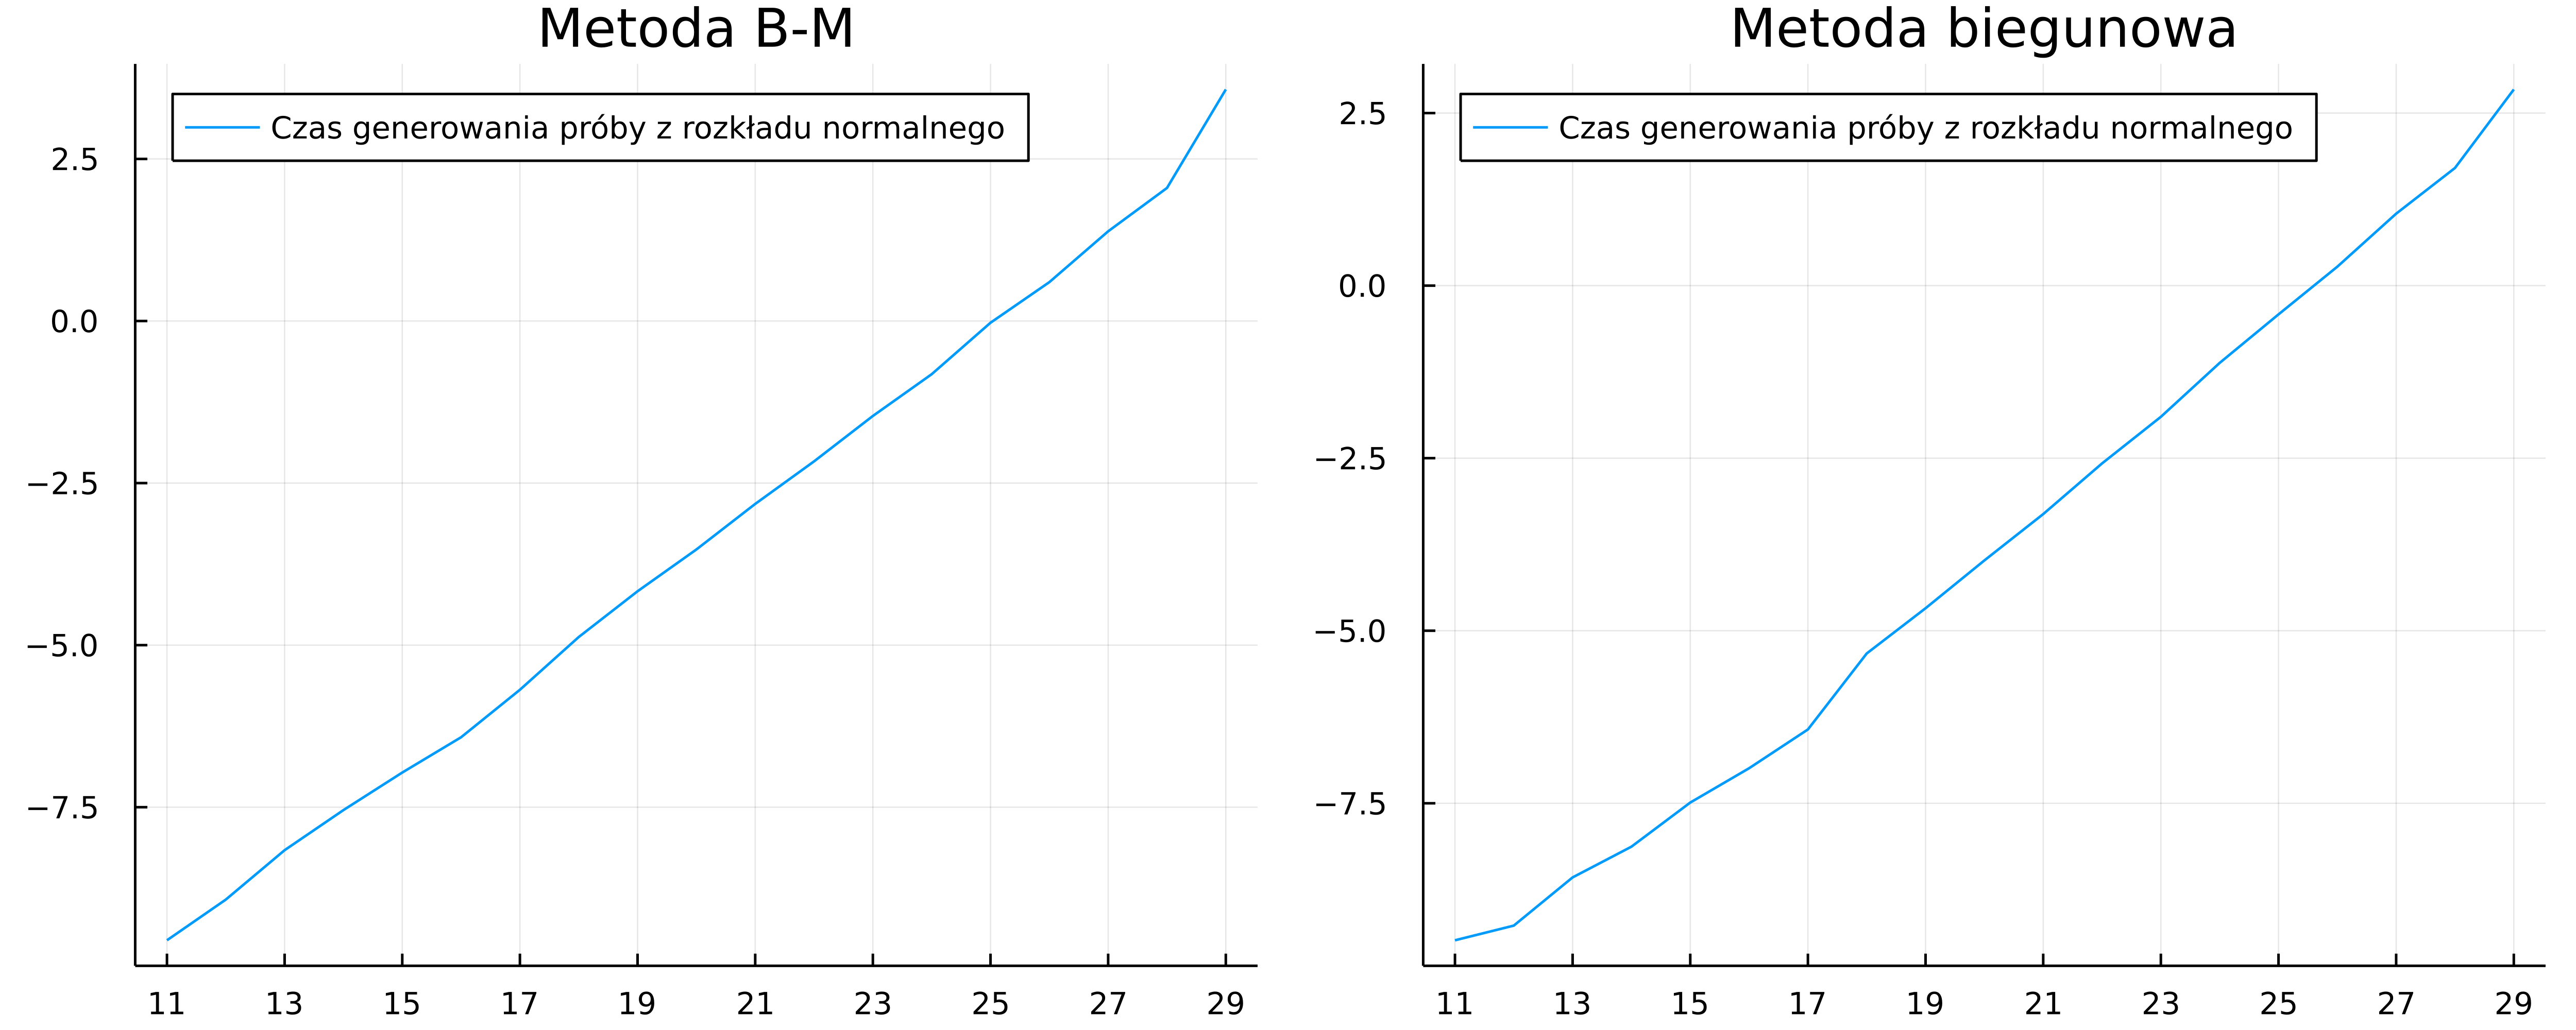
\includegraphics[width=\columnwidth]{fig/fig_normal_time.png}
	\end{figure}
%	\noindent Widzimy, że oba wykresy układają się w linię prostą, więc czas zależy liniowo od wielkości próby.
%	Dodatkowo możemy zauważyć, że na wykresie metody biegunowej pojawiła się jedna dodatkowa wartość dla $n=2^{30}$. Metoda B-M nie zawiera pomiarów dla tej wielkości, ponieważ wielkości tej próby jest za duża by pomieścić ją w pamięci naszych komputerów.
	\noindent Widzimy, że oba wykresy przypominają linię prostą, zatem możemy przypuszczać, że nasze algorytmy mają złożoność czasową rzędu $o(x^n)$, gdzie $n$ jest współczynnikiem kierunkowym powyższych wykresów. Z niewielkimi odchyleniami możemy obliczyć, że $n\approx 1$, z czego wynika, że czas działania obu algorytmów rośnie liniowo wraz z wielkością próby.

	
	\section{Podsumowanie}
	Przedstawiliśmy wszystkie znane nam metody generowania zmiennych losowych. Każdą z metod opisaliśmy
	
	
	
	
	
	
	\begin{thebibliography}{1}
		\bibitem{OD - dyskretny}
		\url{https://www.youtube.com/watch?v=oJYFlu2oJQE}
		
		\bibitem{OD - ciągły}
		\url{https://www.youtube.com/watch?v=NFmbgbyj5M0}
		
		\bibitem{AO - dyskretny}
		\url{https://youtu.be/NFmbgbyj5M0?t=1323}
		
		\bibitem{AO - ciagly}
		\url{https://youtu.be/SpPS0CnhvrE?t=37}
		
		\bibitem{splot}
		\url{https://youtu.be/SpPS0CnhvrE?t=4081}
		
		\bibitem{kompozycja}
		\url{https://youtu.be/7lOH982wrwo?t=50}
		
		\bibitem{box-kox}
		\url{https://youtu.be/7lOH982wrwo?t=1896}
		
		\bibitem{polar}
		\url{https://youtu.be/7lOH982wrwo?t=3349}

	\end{thebibliography}
	
\end{document}